\documentclass{report}
\usepackage{tikz}
\usepackage{graphicx}
\usepackage{relsize}
\usepackage{multirow}
\usepackage{amsmath,amsfonts,amssymb,amsthm,hyperref}
\usepackage{slashed}
\usepackage{graphicx}
\usepackage[compat=1.1.0]{tikz-feynman}
\usepackage{biblatex}
\setlength{\unitlength}{1mm}
\addbibresource{cite.bib}
\newcommand{\nn}{\nonumber}
\allowdisplaybreaks
\numberwithin{equation}{section}
\author{Lê Văn Dũng}
\usepackage[a4paper,left=3cm,right=3cm,top=2.5cm,bottom=2.5cm]{geometry}
\date{July 2021}
\title{REVIEW OF THE STANDARD MODEL}
\begin{document}
\thispagestyle{empty}
\begin{titlepage}
   \begin{center}
       \vspace*{1cm}
    \includegraphics[width=0.5\textwidth]{logo.png}\\
     \begin{huge}  
            Ho Chi Minh City University of Science\\
       Department of Theoretical Physics\\
       July 2021\\
        \vspace{1cm}
       \textbf{ Zh production at lepton collider}\\  
\end{huge}  


       \vspace{0.5cm}
            
       \vspace{1.5cm}
     	 	\begin{Large}  
            \textit{       A thesis presented for the degree of\\
       Bachelor of Science}

		\end{Large} 

       \vfill

            	 	\begin{Large}  
        Student: LE Van Dung\\
       Supervisor: Dr.PHAN Hong Khiem
		\end{Large} 
       \vspace{0.8cm}

            
   \end{center}
\end{titlepage}
\chapter*{Acknowledgement}
\addcontentsline{toc}{chapter}{Acknowledgement}
Firstly, I would like to express my gratitude toward my supervisor Dr.Phan Hong Khiem for his professional guidance. Thank to him, I have been able to develope some insight on proffessional researching and expand my knowledge about the field.

Secondly, I would like to thank my class mates, my friends for accopanying me thoughout the tough but meaningful years of study. Thanks miss My Hau for some of the happiest time of my life, eventhough it is short, I am sure will remember it. 

Thirdly, I would like to thank Dr.Vo Quoc Phong for his sharing and caring he have been doing for my class. The same appreciation to all the teachers of Theoretical Physics department for spreading wonderful klowledge of physics to me and my friends.

Lastly, I thank my family for all their support on every of my decicions   that I made.
\begin{flushright}
\parbox{5cm}{\begin{center}
Ho Chi Minh City, July 17, 2021\\[0.25cm]
LE Van Dung\\
\end{center}
}
\end{flushright}
\chapter*{Abstract}
\addcontentsline{toc}{chapter}{Abstract}
The purpose of this thesis is to study the production of $Z$ boson and Higgs particle at the lepton collider at tree level. We calculate the cross-section of $e^+ + e^-\rightarrow (Z) \rightarrow Z H$ process  in the scope of Standard Model, which yields matching result with \cite{Denner:1992bc}. We also calculate the cross-section of $e^+ + e^-\rightarrow (Z,Z') \rightarrow Z H$ process in the extended $B-L$ model. Most of the calculation is done using $Package-X$ and $Mathematica$. The extended model can be tested can be tested when we have the experimental result from future lepton collider.
\tableofcontents
\chapter{An overview of The Standard Model}
\section{Standard model definition and gauge theory}
The Standard Model is a theory that describes fundamental interactions, base on the symmetry group $SU(3)_c \otimes SU(2)_L \otimes U(1)_Y$. It describe strong, weak, electromagnetic interactions via the exchange of the corresponding spin-1 gauge fields; 8 massless gluons and 1 massless photon, respectively, for the strong and electromagnetic interactions, and 3 massive bosons, $W^\pm$ and $Z$, for the weak interaction. The fermions are classified into 3 generations.
\begin{table}[h]
\centering
\begin{tabular}{|l|l|l|l|}
\hline
generation               & I       & II        & III        \\ \hline
\multirow{2}{*}{leptons} & $e$     & $\mu$     & $\tau$     \\ \cline{2-4} 
                         & $\nu_e$ & $\nu_\mu$ & $\nu_\tau$ \\ \hline
\multirow{2}{*}{quarks}  & $u$     & $c$       & $t$        \\ \cline{2-4} 
                         & $d$     & $s$       & $b$        \\ \hline
\end{tabular}
\caption{Three generations of lepton and quarks}
\end{table}

The gauge invariance is a principle that allow the construction of the interaction between fermions and gauge bosons as well as gauge bosons self-interaction. It is the generalization of the Abelian gauge symmetry found in Quantum Electrodynamics to the non-Abelian case.
\subsection{A historical approach of gauge theory}
The term $gauge$ refers to any specific mathematical formalism to regulate redundant degrees of freedom in the Lagrangian. In Physics, the redundancy originated from Quantum Electrodynamics, more specifically from the Lagrangian for Maxwell’s equations
\begin{equation}
\mathcal{L}=-\frac{1}{4} F_{\mu \nu}F^{\mu \nu},
\end{equation}
with the field strength
\begin{equation}
F_{\mu \nu}=(\partial_\mu A_\mu-\partial_\nu A_\mu).
\end{equation}
The equations of motion that follow Maxwell's Lagrangian is then
\begin{equation}
    \partial_\mu\left[ \frac{\partial \mathcal{L}}{\partial(\partial_\mu A_\nu)}\right]=-\partial^\mu F_{\mu \nu}=0
\end{equation}
The field strength is invariant under the a large group of transformation
\begin{equation}
A_\mu(x)\rightarrow A_\mu(x) +\partial_\mu \lambda(x),
\end{equation}
for any function of $\lambda(x)$.
The equations of motion also mean
\begin{equation}
    [\eta_{\mu\nu}(\partial^\rho \partial_\rho)-\partial_\mu \partial_\nu]A^\mu=0,
\end{equation}
which vanish for any function of the form $\partial_\mu \lambda(x)$, which mean $A_\mu$ and $A_\mu +\partial_\mu \lambda$ are indentified as a same physical state. The degree of freedom of photon is 2 which is called polarization states, while $A_\mu$ field has 4, the symmetry doesn't help us reduce constrain the $A_\mu$ field enough and is to be viewed as a redundancy, thus the transformation take the name $gauge$ $transformation$.\\
We then set constraint on the transformation, or chose a specific gauge, or $gauge-fixing$ to solve the equation of motion. There are a lot of way to chose a gauge such as $Lorrentz$ $gauge$ $\partial_\mu A^\mu=0$, $Coulomb$ $gauge$ $\nabla A_\mu=0$, $Landau$ $gauge$.
Having gauge problem solved, we then construct a interacting theory of light and matter. A direct way of generating interacting term is through Yukawa coupling, we can write 
\begin{equation}
    \mathcal{L}=-\frac{1}{4}F_{\mu\nu}F^{\mu\nu}+ j_\mu A^\mu,
\end{equation}
where $j_\mu$ is some function of matter field, thus the equation of motions read
\begin{equation}
    \partial_\mu F^{\mu\nu}=j^\nu,
\end{equation}
we can set the condition
\begin{equation}
    \partial_\mu j^\mu=0,
\end{equation}
so $j_\mu$ is identified as a conserved current. We might begin with substituting $j_\mu$ with vector current of the fermion field $j^\mu_V=\overline{\psi} \gamma^\mu \psi$,
\begin{equation}
    \mathcal{L}=-\frac{1}{4}F_{\mu\nu}F^{\mu\nu}+\overline{\psi}(\slashed{\partial}-m) \psi+ e\overline{\psi} \gamma_\mu A^\mu \psi,
\end{equation}
here we have introduce a coupling constant $e$. Since Maxwell's Lagrangian have gauge symmetry, it have to also hold for our interacting Lagrangian above, and surprisingly it also does. To see this, we rewrite the Lagrangian as
\begin{equation}
        \mathcal{L}=-\frac{1}{4}F_{\mu\nu}F^{\mu\nu}+\overline{\psi}(\slashed{D}-m) \psi,
\end{equation}
with the covariant derivative $D_\mu=\partial_\mu+ ie  A_\mu $. The transformation of gauge symmetry is
\begin{equation}
    A_\mu(x)\rightarrow A_\mu(x) +\partial_\mu \lambda(x) \quad \text{and} \quad \psi\rightarrow e^{-ie\lambda(x)},
\end{equation}
for any arbitrary function of $\lambda(x)$. The difficulty arises when the derivative acting on $\psi$, since under gauge symmetry, field at different points in space can take on independent phases $\lambda(x)$'s, but everything susprisingly works out, to see this ,we write
\begin{align}
    D_\mu \psi=&(\partial_\mu+ ie  A_\mu) \psi\nn\\
   &\rightarrow \partial_\mu (e^{-ie\lambda}\psi)+ ie (A_\mu(x) +\partial_\mu \lambda) (e^{-ie\lambda}\psi)\nn\\
   &=e^{-ie\lambda} D_\mu \psi,
\end{align}
so the covariant derivative transforms in a nice way as a field does under gauge transformation, paring with $\slashed{\psi}\rightarrow \slashed{\psi}e^{ie\lambda}$, we then have a gauge invariant interacting theory of light and fermions.\\
There is one more thing to note that a true symmetry of a system take one physical state to another with a same properties and result in a consevred current through Noether's theorem.  Gauge symmetry is the redundancy of the system, takes us to nowhere . In QED, there exist a symmetry where $\psi\rightarrow e^{-ie\lambda}\psi$, that result in the conservation of electric charge $e$. The symmetry lies among the infinite gauge symmetry that is $\lambda=constant$.
\subsection{principles of gauge invariance}\label{gaugeinvariant}
\subsubsection{Abelian case}
Gauge invariant originated from
Maxwell theory, when interacting with another fermion field, the
symmetry must hold for the interacting theory. Since QED is gauge
invariant, we might assume that gauge invariant is fundamental and one should construct a theory base on it. We can see that QED is only a trivial example of gauge theory and more theory arises from the more general treatment of gauge theory.\\
Let's say if we want to compare a field at 2 different points $x$ and $y$ , in a local theory, the freedom of gauge symmetry allow the phase chosen at $x$ is independent of that at $y$, then we would have
\begin{equation}
    \psi(y)-\psi(x)\rightarrow e^{i\alpha(y)}\psi(y)- e^{i\alpha(x)}\psi(x),
\end{equation}
the difference depends on our choice of local phase $\alpha(y)$ and $\alpha(x)$ thus make comparing field value 2 different point unclear, for instance, $|\psi(x)-\psi(y)|$ depends on our choice of local phase. The factor $\partial_\mu \psi$ is there for cannot be compute since derivative involves subtracting field values at 2 different points.\\
To make comparing field at 2 different points well defined, a new field is introduced $W(x,y)$, named Wilson line. It is a kind of
bi-local field that depends on two points \cite{Schwartz:2014sze}. The field transform as
\begin{equation}
    W(x,y)\rightarrow e^{i\alpha(x)} W(x,y)e^{-i\alpha(y)},
    \label{wilson}
\end{equation}
so that
\begin{align}
    [W(x,y)\psi(y)-\psi(x)]&\rightarrow  e^{i\alpha(x)} W(x,y)e^{-i\alpha(y)}e^{i\alpha(y)}\psi(y)-e^{i\alpha(x)}\psi(x)\nn\\
    &=e^{i\alpha(x)}[W(x,y)\psi(y)-\psi(x)],
\end{align}
now the quantity $|W(x,y)\psi(y)-\psi(x)|$ is now independent of our choice of local field. Taking $x^\mu=x^\mu+ \delta x^\mu$, divide by $\delta x^\mu$, $\delta x^\mu \rightarrow 0$, we can turn the difference into a new form of derivative
\begin{equation}
    D_\mu\psi=\lim_{\delta x\rightarrow 0} \frac{W(x,x+\delta x)[\psi(x+\delta x)-\psi(x)]}{\delta x^\mu},
    \label{covariantder}
\end{equation}
then 
\begin{equation}
    D_\mu \psi(x) \rightarrow  e^{i\alpha(x)} D_\mu \psi(x).
\end{equation}
when $x^\mu=y^\mu$, means there is no separation, $W(x,x)$ should be equal to 1. We can expand the field around $\delta x^\mu$
\begin{equation}
W(x,x+\delta x)= 1- i e A_\mu(x)\ \delta x^\mu+ \mathcal{O}(\delta x^\mu)+ ...,    
\end{equation}
where $e$ is arbitrary constant. Then $A_\mu$ follow the transformation \eqref{wilson} that
\begin{align}
W(x,x+\delta x)&\rightarrow   e^{i\alpha(x)} W(x,x +\delta x)e^{-i\alpha(x+\delta x)}\nn\\
\Rightarrow 1- i e A_\mu(x)\ \delta x^\mu &\rightarrow  e^{i\alpha(x)}[1- i e A_\mu(x)\ \delta x^\mu] e^{-i\alpha(x+\delta x)}\nn\\
\Rightarrow 1- i e A_\mu(x)\ \delta x^\mu &\rightarrow  e^{i\alpha(x)}[1- i e A_\mu(x)\ \delta x^\mu] e^{-i\alpha(x)}[1- i\delta x \partial_\mu \alpha(x)]\nn\\
\Rightarrow i e A_\mu(x)\ \delta x^\mu &\rightarrow  i e A_\mu(x)\ \delta x^\mu- i\delta x \partial_\mu \alpha(x)+e \delta x^2 A_\mu(x)\partial_\mu \alpha(x)\nn\\
\Rightarrow  A_\mu(x) &\rightarrow  A_\mu(x)- \frac{1}{e} \partial_\mu \alpha(x).
\end{align}
Follow \eqref{covariantder} we have
\begin{equation}
D_\mu \psi= (\partial_\mu- ie A_\mu) \psi,
\end{equation}
The field $A_\mu$ is introduced as a \textbf{connection}, allow us to compare the field values at different point despite their arbitrary phases.\\
The particular expression of $W(x,y)$ is 
\begin{equation}
W_P(x,y)=\exp \left( ie\int_y^x A_\mu (z)dz^\mu \right) ,
\end{equation}
this functional of $A_\mu$ is called \textbf{Wilson line}. The integral is a line integral along any path $P$ form $y^\mu$ to $x_\mu$. More details discussion is in \cite{Schwartz:2014sze}.
Note that $D_\mu \psi$ transform just like $D_\mu D_\nu$ and so 
\begin{equation}
[D_\mu ,D_\nu]\psi \rightarrow e^{i\alpha(x)}[D_\mu ,D_\nu]\psi,
\end{equation}
and we also have
\begin{equation}
[D_\mu ,D_\nu]\psi= -ie F_{\mu\nu} \psi,
\end{equation}
$[D_\mu ,D_\nu]$ turns out to be a function instead of an operator. We can define QED field strength as
\begin{equation}
F_{\mu\nu}\equiv \frac{i}{e}[D_\mu ,D_\nu].
\end{equation}
Now we have local $U(1)$ invariant Langrangian base on Dirac Lagrangian
\begin{equation}
\mathcal{L}=i\overline{\psi}\gamma^\mu D_\mu \psi+m\overline{\psi}\psi
-\frac{1}{4} F_{\mu \nu} F^{\mu \nu}.
\end{equation}
We can see that the existence of the 
gauge field $A_\mu$ is a consequence of local symmetry: without it we could not 
write an invariant Lagrangian involving derivatives of $\psi$, or compare the values of 2 field.
\subsubsection{Non-Abelian case}
Non-Abelian case of gauge symmetry is more than a phase rotation. let's us start with kinetic terms of $N$ Dirac massless fermions
\begin{equation}
\mathcal{L}=\sum^N_j i\overline{\psi}_j \gamma^\mu \partial_\mu \psi_j,
\end{equation}
this Lagrangian is invariant under $SU(N)$ global transformation
\begin{equation}
\psi_j\rightarrow (e^{i\alpha^a T^a})_{ij} \psi_j,
\end{equation}
where $T^a$ are the generators of $SU(N)$ in the fundamental representation. The symmetry is called global because $alpha^a$ does not depend on $x$. Now we require $SU(N)$ symmetry to be local, i.e., $\alpha$ depends on x, the treatment of the field comparison is just as before, where we introduce new field $W(x,y)$,
\begin{equation}
W(x^\mu,x^\mu+\delta x^\mu)=\normalfont\hbox{1\kern-0.15em \vrule width .8pt depth-.5pt}-ig \textbf{A}_\mu \delta x^\mu,
\end{equation}
with the field
\begin{equation}
\textbf{A}_\mu= A_\mu^a T^a,
\end{equation}
which mean for every generator correspond to one gauge field.
The local unitary transformation is $U(x)=e^{i\alpha^a T^a}\ \in SU(N)$, field transform is written as
\begin{equation}
\vec{\psi}\rightarrow U(x) \vec{\psi},
\end{equation}
and for the Wilson line
\begin{equation}
 W(x,y)\rightarrow U(x) W(x,y)U^\dagger (y).
\end{equation}
To see how $A_\mu^a$ transform, we can start from $D_\mu \vec{\psi}\rightarrow U \cdot D_\mu \vec{\psi}$, so we have 
\begin{equation}
(\partial_\mu-ig\textbf{A}'_\mu)\cdot U \cdot \vec{\psi}\rightarrow U\cdot (\partial_\mu-ig\textbf{A}_\mu)\cdot \vec{\psi},
\end{equation}
where $\textbf{A}_\mu'$ is transformed field, so
\begin{equation}
ig\textbf{A}_\mu'\cdot U=ig U\cdot \textbf{A}_\mu+\partial_\mu U,
\end{equation}
and we now have the transformation for the gauge field
\begin{equation}
\textbf{A}_\mu'=ig U\cdot \textbf{A}_\mu U^{-1}+\frac{i}{g} (\partial_\mu U) A^{-1}.
\end{equation}
In terms of infinitesimal transformation, we have
\begin{equation}
A_\mu^a \rightarrow A_\mu^a + \frac{1}{g}\partial_\mu \alpha^a(x)- f^{abc} \alpha^b(x)A_\mu^c.
\end{equation}
The commutation is now
\begin{equation}
[D_\mu,D_\nu]\psi=(-ig (\partial_\mu\textbf{A}-\partial_\mu\textbf{A}_\nu)-g^2[\textbf{A}_\mu,\textbf{A}_\nu])\psi,
\end{equation}
which means
\begin{equation}
\textbf{F}_{\mu\nu}=\frac{i}{g} [D_\mu,D_\nu]
\end{equation}
or
\begin{equation}
F_{\mu\nu}^a=(\partial_\mu A-\partial_\mu A_\nu)-gf^{abc}A_\mu A_\nu.
\end{equation}

\subsection{$SU(3)_c$ symmetry}
Quantum chromodynamics is a non-abelian gauge theory, with the symmetry group SU(3) describing strong interaction between quarks and gluons, the fundamental particles that make up mesons and hadrons. Mesons are made up from 2 quarks as $q\overline{q}$ state, hadrons are made up from 3 quark as $qqq$ states. In order to satisfy Pauli's Exclusion Principle, quarks have to have a new quantum number, $color$, such that each species of quark may have 3 different colors.
A color state is a combination of 3 colors $\alpha= red(r), green(g), blue(b)$
\begin{equation}
|\psi \rangle = \alpha_1 |r\rangle +\alpha_2 |g\rangle+ \alpha_3 |b\rangle=\begin{pmatrix}
\alpha_1\\\alpha_2\\\alpha_3\\
\end{pmatrix}
\end{equation}
with $\alpha_i$ are the coefficients and the basis vectors that span the color space are
\begin{equation}
|r\rangle=\begin{pmatrix}
1\\0\\0
\end{pmatrix}\quad |g\rangle=\begin{pmatrix}
0\\1\\0
\end{pmatrix}\quad |b\rangle \begin{pmatrix}
0\\0\\1
\end{pmatrix}.
\end{equation}
We denote $q_f^\alpha$ a quark field with flavor $f$ and color $\alpha$. To simplify the equation, let us adopt a vector in color space: $q^T_f \equiv (q^{\alpha_1},q^{\alpha_2},q^{\alpha_3})$.\\
The  Lagrangian 
\begin{equation}
\mathcal{L}_0=\sum_f \overline{q}_f(i\gamma^\mu \partial_\mu-m_f)q_f
\end{equation} 
is invariant under arbitrary global $SU(3)_C$ transformation in color space
\begin{equation}
q^\alpha_f \xrightarrow{} (q_f^\alpha)'= U^\alpha_\beta q^\beta_f. \quad\quad UU^\dagger= U^\dagger U = 1 \quad\quad \text{det}U=1.
\end{equation}
The $SU(3)_C$ transformation matrices can be written in the form
\begin{equation}
U=exp\left( i\sum_a \phi_a\frac{\lambda^a}{2}\right),
\end{equation}
where $\frac{1}{2}\lambda^a (a=1,2,...,8)$ denote the 8 generators of the fundamental representation of the $SU(3)_c$ algebra, $\phi_a$ are free parameters. The matrices $\lambda^a$ satisfy  the commutation 
\begin{equation}
\label{commut}
\left[\frac{\lambda^a}{2},\frac{\lambda^b}{2}\right] = i f^{abc} \frac{\lambda^c}{2},
\end{equation}
with $f^{abc}$ are the $SU(3)_C$ structure constants.
Analogous to the QED case, we can now require the Lagrangian to be also invariant under local $SU(3)_C$ transformation, $\phi_a =\phi_a(x)$. To satisfy this requirement, we need to change the quark derivatives by covariant derivative. Since we now have eight independent generators of the $SU(3)_c$ group, eight different gauge bosons, which are so-called gluons are needed:
\begin{equation}
 D^\mu q_f \equiv \left[\partial^\mu - i g_s\frac{\lambda^a}{2}G^\mu_a(x)\right] q_f,
 \end{equation} 
 where $g_s$ is the the coupling constant.
The covariant derivative of the field transform exactly the same way as the color-vector $q_f$, this keep the transformation property of the the field:
\begin{equation}
(D^\mu)'=U D^\mu U^\dagger \quad \text{and}\quad G^\mu \rightarrow (G^\mu)'= UG^\mu U^\dagger -\frac{i}{g_s}(\partial^\mu U)U^\dagger.
\end{equation}
The transformation of the gluon fields is more complicated than the one obtained from the QED case. The non-commutativity of the $SU(3)_C$ matrices give rise to the additional self-interacting terms of the gluon fields them self.
\subsection{$SU(2)_L\otimes U(1)_Y$ symmetry}
Using gauge invariance, we have been able to determine the QED and QCD Lagrangians. For weak interaction, let us start with Dirac Lagrangian for $N$ free fermion field
\begin{equation}
    \mathcal{L}=i\overline{\psi}_j\slashed{\partial} \psi_j+m\overline{\psi}_j\psi_j,
\end{equation}
if we ignore the mass and set it to 0, the Lagrangian can be split into
left-handed and the right-handed  Weyl spinors which are completely decoupled, we can treat $\psi_L$ and $\psi_R$ as 2 different species of field,
\begin{equation}
    \mathcal{L}=\psi^\dagger_{jL}\ i \overline{\sigma}\cdot \partial \psi_{jL}+\psi^\dagger_{jR}\ i \sigma\cdot \partial \psi_{jR},
\end{equation}
rotating the left-handed and the right-handed components independently makes no difference to the Lagrangian
\begin{equation}
\psi_{jL}\xrightarrow{left}e^{i\theta_L} \psi_{jL} \quad \text{and} \quad \psi_{jR}\xrightarrow{left}\psi_{jR},
\end{equation}
or
\begin{equation}
\psi_{jL}\xrightarrow{right}\psi_{jL} \quad \text{and} \quad \psi_{jR}\xrightarrow{right}\phi^{i\theta_R}\psi_{jR},
\end{equation}
since left and right handed fields lie in different representation, i.e., $(\frac{1}{2},0)$ for left-handed spinor, $(0,\frac{1}{2})$ for right handed spinor, we have no trouble coupling  only left-handed field to a gauge field. \\
\begin{equation}
    \mathcal{L}=\psi^\dagger_{jL}\ i \overline{\sigma}\cdot D \psi_{jL}+\psi^\dagger_{jR}\ i \sigma\cdot \partial \psi_{jR},
\end{equation}
with $D_\mu=\partial_\mu -igA_\mu^aT^a$. we can Lagrangian above rewrite this in terms of Dirac spinors as
\begin{align}
    \psi &\rightarrow \left( 1+ i \alpha^a t^a P_L\right)\psi,\\
    A_\mu^a&\rightarrow A_\mu^a +\frac{1}{g}\alpha^a+f^{abc} A_\mu^b A_\nu^c,
\end{align}
with $\psi=(\psi_1,\psi_2,...)^T$ are a set of $N$ Dirac fermions, $t^a$ are generators of the symmetry group in the fundamental representation.\\
We have free theory of $N$ complex fields is automatically invariant under $SU(N)\times U(1)$, in this case $N=2$. The actual larger symmetry group is  $SU(N)_L\times SU(N)_R\times U(1)_V\times U(1)_A$, where 2 $U(1)$ symmetry are \textbf{vector} and \textbf{axial}. The vector symmetry accounts for, in this case, conservation of lepton number. The axial symmetry is broken by a quantum effects called anomalies. Nature only chose gauge fields to couple to left-handed fields, so we can derive the coupling by letting left-handed components of quark and lepton to be in variant under $SU(2)$, this symmetry is named $SU(2)_L$ because of it, thus the doublets are
\begin{equation}
\psi_L: Q_L=\begin{pmatrix}
    u\\d
    \end{pmatrix}_L, \quad L_L=\begin{pmatrix}
    \nu\\e
    \end{pmatrix}_L,
\end{equation}
which will be couple to the gauge fields called $W$ bosons. The right-handed fields remain as singlet under $SU(2)_L$ transformations
\begin{align}
\psi_R(x):  \nu_{eR},e_R,u_R,d_R,
\end{align}
soon later, 2 more generations of fermions are added to the Lagrangian to form electroweak theory.
A simplier way of writing the transformation of left-handed fields is:
\begin{align}
&\psi_L(x)\xrightarrow{G}\psi'_L(x)= \exp(i Y\beta) \ \exp(i\frac{\sigma_i}{2}\alpha^i) \ \psi_L(x)\\
&\psi_R(x)\xrightarrow{G}\psi'_R(x)= \exp(iY\beta)  \ \psi_R(x),
\end{align}
where the $SU(2)_L$ transformation is
\begin{equation}
 U_L=\exp(i\frac{\sigma_i}{2}\alpha^i)\quad (i=1,2,3)
 \end{equation}
the right-handed fields act like a singlet under $U_L$ so there is no need to include it in. $Y$ and $T_i=\frac{\sigma_i}{2} \ ,(i=1,2,3)$  are the generators of $U(1)_Y $ and $SU(2)_L $ respectively. The parameter $Y $ is called hypercharges (named after the electric charge $Q$ analogous to the QED gauge coupling) . The hyper charge $Y$ is totally free in this case, meaning that it can take on any value, but we will find that it and electric charge $Q$ are related to each other via Gell-man-Nishijima formula: $T^3 +Y=Q$ in the next section.

We now can require the Lagrangian to be invariant under $SU(2)_L\otimes U(1)_Y$ local transformations. In order to satisfy this symmetry requirement, we need to change the the fermion derivatives with the covariant ones, since we have four independent generators, we need four gauge bosons for the covariant derivative:
\begin{align}\label{2}
&D_\mu[\psi_L(x)]\equiv \partial_\mu -ig\frac{\sigma^i}{2}W^\mu_i(x)- ig'YB_\mu(x),\\
&D_\mu[\psi_R(x)]\equiv \partial_\mu - ig'YB_\mu(x),
\end{align}
and so we have the transformation of the gauge fields:
\begin{align}
&B_\mu(x) \rightarrow B'_\mu(x) =B_\mu(x)+\frac{1}{g'}\partial_\mu \beta(x).\\
&W_\mu^i \rightarrow (W_\mu^{i})'=U_L(x)W_\mu^iU_L^\dagger(x)- \frac{i}{g}U_L(x) U_L^\dagger(x).
\end{align}
The Lagrangian is now becomes
\begin{equation}
\label{eqn:Ferm}
\mathcal{L}=\sum_i i\overline{L}^j\gamma^\mu D_\mu L^j + i\overline{Q}^j_L\gamma^\mu D_\mu Q^j_L + i\overline{\psi}^j_R\gamma^\mu D_\mu \psi^j_R,
\end{equation}
which is invariant under the $SU(2)_L\times U(1)_Y$ transformation,
the superscript $i$ runs over three generations of fermion.
The Lagrangian (\ref{eqn:Ferm}) contains the interaction between the fermion fields and the gauge bosons
\begin{equation}
\mathcal{L}\quad \subset \quad g\overline{\psi}_L \gamma^\mu W_\mu^i \psi_L +g'\overline{\psi}_L \gamma^\mu B_\mu \psi_L+ g'B_\mu \overline{\psi}_R\gamma^\mu B_\mu \psi_R,
\end{equation}
Left and right handed fermions are considered to be independent under massless theory, but a massive fermions is a combination of 2 helicity of the massless theory, thus they are connected in some ways.
\section{Standard Model Lagrangian}
The SM Lagrangian 
\begin{equation}
\mathcal{L}_{SM}=\mathcal{L}_{Fermion}+\mathcal{L}_{gauge}+\mathcal{L}_{Higgs}+\mathcal{L}_{Yukawa}
\end{equation}
consists of 4 major sectors which are the fermion kinetic sector $\mathcal{L}_{Fermion}$, the gauge field kinetic sector $\mathcal{L}_{gauge}$, the Higgs field sector $\mathcal{L}_{Higgs}$, the Yukawa sector $\mathcal{L}_{Yukawa}$.
\subsection{Fermion Lagrangian}
The fermion Lagrangian
\begin{equation}
\begin{split}
\mathcal{L}_{Fermion}=\sum_j \mathcal{L}_0 = i\overline{L}^j(x) \gamma^\mu \partial_\mu L^j(x)+i\overline{Q}_L^j(x) \gamma^\mu \partial_\mu Q_L^j(x)+\\
i\overline{e}_R^j(x) \gamma^\mu \partial_\mu e_R^j(x)+
i\overline{u}_R^j(x) \gamma^\mu \partial_\mu u_R^j(x)+
i\overline{d}_R^j(x) \gamma^\mu \partial_\mu d_R^j(x),
\end{split}
\end{equation}
is the source where interactions between fermions and gauge bosons appear, but in this form, the physical contents haven't transparent yet.
The superscript $j$ denote generation of the fermions. The covariant for the left and right fields are:
\begin{align}
&D_\mu[\psi_L(x)]\equiv \partial_\mu -ig\frac{\sigma^i}{2}W^\mu_i(x)- ig'YB_\mu(x),\\
&D_\mu[\psi_R(x)]\equiv \partial_\mu - ig'YB_\mu(x).\\
\end{align}
\subsection{Yang-Mills Lagrangian, gauge fields kinetic terms\label{12}}
We did indeed construct a gauge invariant terms of the gauge fields in \ref{gaugeinvariant}, now we simply state
\begin{align}
\textbf{F}_{\mu\nu}&=\frac{i}{g}\left[D_\mu,D_\nu\right],\\
[D_\mu,D_\nu]&=(-ig (\partial_\mu\textbf{A}-\partial_\mu\textbf{A}_\nu)-g^2[\textbf{A}_\mu,\textbf{A}_\nu])\\
\end{align}
or
\begin{equation}
    F_{\mu\nu}^a=\partial_\mu A_\nu^a-\partial_\mu A^a_\nu +f^{abc} A_\mu^b A_\nu^c
\end{equation}
where $t^a$ are generators of the 
symmetry group in the fundamental representation, $f^{abc}$ is a set of numbers called structure constants, $\textbf{F}_{\mu\nu}=F_{\mu\nu}^a t^a$, $\textbf{A}_\mu=A_\mu^aT^a$. Consider an electromagnetic field $A_\mu^a$, we can write more explicitly:
\begin{equation}
F_{\mu\nu}^a=\partial_\mu A_\nu^a -\partial_\nu A^a_\nu ,
\end{equation}
$f^{abc}=$ since the symmetry is Ablelian.
gauge-invariant terms can be generate from combinations of the field strengths:
\begin{equation}
\mathcal{L}=-\frac{1}{4}(F_{\mu\nu}^a)^2= -\frac{1}{2} Tr \left[\left(F_{\mu\nu}^a t^a\right)^2\right].
\end{equation}
Now we can apply this to find the field strength  of the gauge bosons we have mentioned so far::
\begin{align}
&G_{\mu\nu}^a=\partial_\mu G_\nu^a -\partial_\nu G^a_\mu +g_c f^{abc} G_\mu^b G_\nu^c\\
&W_{\mu\nu}^a=\partial_\mu W_\nu^a -\partial_\nu W^a_\mu +g \epsilon^{abc} W_\mu^b W_\nu^c \label{13}\\
&B_{\mu\nu}=\partial_\mu B_\nu -\partial_\nu B_\mu \label{14} ,
\end{align}
thus we have the kinetic term for the gauge fields :
\begin{equation}
\mathcal{L}_{gauge}= -\frac{1}{4}B_{\mu\nu}B^{\mu\nu}
-\frac{1}{4}W_{\mu\nu}^iW^{\mu\nu}_i-\frac{1}{4}G_{\mu\nu}^iG^{\mu\nu}_i
\end{equation}
Due to the non-commutativity of the generator of the $SU(2)_L$ and $SU(3)_C$, the kinetic term gives rise to cubic and
quartic self-interactions among the gauge fields.
\subsection{Higgs Lagrangian and Spontaneous symmetry breaking }
SSB happens in a lot of places in physics, the most famous example of SSB is in ferromagnet, where all particles' spin have rotational symmetry at high temperature, when the temperature goes below the Curie temperature,  the particles are at a set of degenerated states which their spins align in some particular direction, thus the rotational symmetry is broken, we can say the field theory has hidden broken symmetry. It is possible that the field takes on a nonzero global value, then the system goes to one of its vacuum minima, the symmetry is broken, note that the true symmetry is hidden in the arbitrary selection of ground state, but we have to work from one of them with the theory. SSB is a important way of generating fermions' mass and their self interactions and later on explain the theory of weak interaction.
\subsubsection{Discrete symmetry}
In the most simple case of SSB, first consider the $\phi^4$ Lagrangian:
\begin{equation}
\label{eqn:classical-ssbL}
\mathcal{L}=\frac{1}{2}(\partial_\mu\phi)^2+\frac{1}{2}\mu^2\phi^2-\frac{\lambda}{4!}\phi^4,
\end{equation}
this Lagrangian is invariant under $\phi=\rightarrow -\phi$ transformation.
The minimum-energy classical configuration is a field $\phi_0$ that minimize the potential
\begin{equation}
V(\phi) = -\frac{1}{2}\mu^2+\frac{\lambda}{4!}\phi^4,
\end{equation}
this potential has two minima at
\begin{equation}
\phi_0=\pm v=\pm \sqrt{\frac{6}{\lambda}}\mu,
\end{equation}
the constant $v$ is called $vacuum\ expectation\ value$ ($VEV$) of $\phi$. We next expand $\phi$ around the positive minimum
\begin{equation}
\label{eqn:phi-sigma}
\phi(x)=v+\sigma(x),
\end{equation}
rewrite $\mathcal{L}$ in terms of $\sigma(x)$,plugging new field expansion to the Lagrangian(\ref{eqn:classical-ssbL})
\begin{equation}
\mathcal{L}=\frac{{\partial_\mu \sigma }^2}{2}-\frac{3 \mu ^4}{2 \lambda }+\frac{\sqrt{{\lambda }}\mu  \sigma ^3}{\sqrt{6} }+\frac{\lambda  \sigma ^4}{24}+\mu ^2 \sigma ^2.
\end{equation}
We find that the term linear in $\sigma$ vanishes. This Lagrangrian describe a scalar field with mass $\sqrt{2}\mu$ and $\sigma^3,\sigma^4$ interactions. The $\phi\rightarrow -\phi $ is broken, this is the simplest example of spontaneous symmetry breaking.
\subsubsection{Continuous symmetry- linear sigma model}
The most important example is the generalization of previous case is the linear sigma model.
The Lagrangian of linear sigma model involves a set of N real scalar fields
\begin{equation}
\label{eqn:linear-ssbL}
\mathcal{L}=\frac{1}{2}(\partial_\mu\phi^i)^2+\frac{1}{2}\mu^2(\phi^i)^2-\frac{\lambda}{4}\left[\sum_i(\phi^i)^2\right]^2
\end{equation}
is invariant under the symmetry
\begin{equation}
\phi^i=R^{ij} \phi^j,
\end{equation}
which is a rotational group in $N$ dimensions, also called the $N-dimensional\ orthogonal\ group$ or simply $O(N)$. The lowest-energy configuration is a constant field $\phi_0^i$ which minimize the potential value
\begin{equation}
V(\phi^i)=
-\frac{1}{2}\mu^2(\phi^i)^2+\frac{\lambda}{4}\left[\sum_i(\phi^i)^2\right]^2,
\end{equation}
the field $\phi^i$ takes on the form of any value that satisfy
\begin{equation}
(\phi^i_2)^2=\frac{\mu^2}{\lambda},
\end{equation}
this condition determines the length of the vector $\phi^i$ in $N$ dimensions. It is conventional to chose a coordinate so that $\phi^i$ points in the $N$th direction :
\begin{equation}
\phi^i=(0,0,...,v) \quad,
\end{equation}
where
\begin{equation}
v=\frac{\mu}{\sqrt{\lambda}}.
\end{equation}
Expand the field around the minima
\begin{equation}
\phi^i=(\pi^k(x),v+\sigma(x)), \quad k=1,2,...,N-1.
\end{equation}
It is now straightforward that we rewrite the Lagrangian in terms of $\pi^k(x)$ and $\sigma(x)$
\begin{equation}
\begin{split}
\mathcal{L}=\frac{(\partial_\mu \sigma) ^2}{2}+\frac{( \partial_\mu \pi )^2}{2}-\frac{\mu ^4}{4 \lambda }+\sqrt{\lambda } \mu  \sigma ^3+\pi ^2 \sqrt{\lambda } \mu  \sigma +\frac{\lambda  \sigma ^4}{4}+\frac{1}{2} \pi ^2 \lambda  \sigma ^2+\frac{\pi ^4 \lambda }{4}+\mu ^2 \sigma ^2,
\end{split}
\end{equation}
we obtain mass of the $\sigma$ field is $\sqrt{2}\mu$, and also a set of $N-1$ massless $\pi$ fields. The original $O(N)$ symmetry is broken leaving behind the $O(N-1)$ symmetry, which is the number of direction in which the field can rotate after acquire VEV.
\subsubsection{Higgs Lagrangian}
Now we combine gauge theories with SSB, starting by replace the partial derivative with covariant derivative in the Lagrangian (\ref{eqn:classical-ssbL})
\begin{equation}
\begin{split}
\label{eqn:L higgs}
&\mathcal{L}_H=(D_\mu\phi)^\dagger D^\mu \phi - V(\phi)\quad \quad\quad\quad V(\phi)=\mu^2 \phi^\dagger \phi + \lambda(\phi^\dagger \phi)^2\\
&D_\mu[\phi(x)]\equiv \partial_\mu -ig\frac{\sigma^i}{2}W^\mu_i(x)- ig'Y B_\mu(x)
\end{split}
\end{equation}
we introduce the new complex scalar field doublet of $SU(2)_L$ with hyper charge $Y=1/2$
\begin{equation}
\phi(x)\equiv \begin{pmatrix}
\phi^{(+)}(x)\\
\phi^{(0)}(x)
\end{pmatrix}
\end{equation}
The Lagrangian is invariant under $SU(2)_L \otimes U(1)_Y$ transformations, and the hypercharge $Y$
.
The lowest-energy configuration is a set of degenerate state of $\phi$ that minimize the potential energy value
\begin{equation}
\phi^\dagger \phi=\sqrt{\frac{-\mu^2}{2 \lambda}}=\frac{v}{\sqrt{2}}
\end{equation}
we can select a real and electrically neutral state, $Q\phi_0=0$
\begin{equation}
\phi_0=\frac{1}{\sqrt{2}}\begin{pmatrix}
0\\
v
\end{pmatrix}
\end{equation}
the $SU(2)_L\otimes U(1)_Y$ symmetry is broken down to $U(1)_{QED}$ symmetry. Now we can expand the field around the minimum of the vacuum 
\begin{equation}
\phi =\frac{1}{\sqrt{2}}\begin{pmatrix}
\chi_1(x)+i \chi_2(x)\\
v +h(x)+ i\chi_3(x)
\end{pmatrix}
\end{equation}
here $\chi_1(x),\chi_2(x),\chi_3(x)$ are massless Goldstone bosons, we can chose a specific $SU(2)_L$ phase transformation (unitarity gauge) of the field so that we can eliminate the Goldstone bosons , thus we have the Higgs doublet field
\begin{equation}\label{7}
\phi=\frac{1}{\sqrt{2}}\begin{pmatrix}
0\\
v+h(x)
\end{pmatrix}
\end{equation}
the field $h(x)$ is a scalar particle with mass
\begin{equation}
m_h=\sqrt{\frac{\lambda}{2}}v
\end{equation}
The expansion of the kinetic term in (\ref{eqn:L higgs}) in unitarity gauge yields the gauge bosons mass term
\begin{equation}
\mathcal{L}_{mass}=\frac{1}{2}\frac{v^2}{4}\left[g^2(W^1_\mu)^2+g^2(A^2_\mu)^2+(-gW_\mu^3+g'B_\mu)^2\right]
\end{equation}
here we make a transformation
\begin{align}
W^{\pm}=\frac{1}{\sqrt{2}}(W_\mu^1\mp W^2_\mu),\\
Z_\mu=c_w W_\mu^3-s_wB_\mu,\\
A_\mu=s_w W_\mu^3-c_w B_\mu,\\
\end{align}
with $s_w=\sin \theta_w, c_w=\cos \theta_w,\tan \theta_w=\frac{g'}{g}$. $\theta_w$ is called the $weak\  mixing\ angle$. From this we can define the mass of the gauge bosons as follow
\begin{align}
m_W&=\frac{gv}{2},\\
m_Z&=\sqrt{g^2+g'^2}\frac{v}{2},\label{8}\\
m_A &= 0.
\end{align}
\subsection{Yukawa Lagrangian, fermion mass term}
The ordinary mass term for Fermion $-m\overline{\psi}\psi = -m(\overline{\psi}_L\psi_R+\overline{\psi}_R\psi_L)$ is not allowed, because the right and left and right handed fermion transform differently under gauge transformation so it break the gauge symmetry, but if the symmetry is spontaneously broken on it self, then the existence of the fermions mass term is possible by associate fermion fields with the Higgs doublet after the symmetry breaking. Yukawa interaction between Higgs field and the fermion fields are then introduced to give mass to the fermions.
\begin{equation}
\begin{split}
\mathcal{L}_Y=&-G_l^{ij}\overline{L}^{i}_L\phi l^{j}_R -G_d^{ij}\overline{Q}^{i}_L\phi d_R^{j}-G_u^{ij}\overline{Q}^{i}_L\phi^c u_R^{j}+h.c,
\end{split}
\end{equation}
here $i,j$ run from 1 to 3 denote the fermion generations, that mean $G_L,G_u,G_d$ are coupling matrices that may include mixing interaction between the generations. For simplicity, Yukawa Lagrangian for one generation of quark $Q_L=(u_L\quad d_L)^T$, leptons $L_L=(\nu_L\quad l_L)^T$, Higgs field $\phi$ and its charge-conjugate $\phi^c=i\sigma^2 \phi=(\phi^{0*},-\phi^-)^T$ with $\phi^{(-)}$ is the adjoint of $\phi^{(+)}$
\begin{equation}
\begin{split}
\mathcal{L}_Y&=-G_l\overline{L}_L\phi l_R -G_d\overline{Q}_L\phi d_R-G_u\overline{Q}_L\phi^c u_R\\
&=-G_l(\overline{\nu}_e,\overline{e})_L\begin{pmatrix}
\phi^{(+)}\\
\phi^{(0)}
\end{pmatrix}e_R-G_u(\overline{u},\overline{d})_L\begin{pmatrix}
\phi^{(0)*}\\
-\phi^{(-)}
\end{pmatrix}u_R-G_l(\overline{u},\overline{d})_L\begin{pmatrix}
\phi^{(+)}\\
\phi^{(0)}
\end{pmatrix}d_R,
\end{split}
\end{equation}
In the unitarity gauge, this Lagrangian takes the simpler form
\begin{equation}
\mathcal{L}_Y=-\frac{1}{\sqrt{2}}(v+h(x))(g_e \overline{e}e+g_u \overline{u}u+g_d, \overline{d}d),
\end{equation}
from this Lagrangian we can filter out the fermion masses:
\begin{equation}
m_e=g_e \frac{v}{\sqrt{2}}, \quad m_u=g_u \frac{v}{\sqrt{2}}, \quad m_d=g_d \frac{v}{\sqrt{2}},
\end{equation}
where $G_e,G_u,G_d$ are Yukawa coupling constants.
\section{Feynman rules for the $e^+ + e^- \rightarrow Z H$}
From the general Lagrangian, we can pick out the terms that involve in our process
\begin{equation}
\begin{split}
\mathcal{L}_{process}=\ &\ i\overline{E}_L\gamma^\mu D_\mu E_R + i\overline{e}_L\gamma^\mu D_\mu e_R
-\frac{1}{4}B_{\mu\nu}B^{\mu\nu}\\
&+(D_\mu\phi)^\dagger D^\mu \phi -\mu^2 \phi^\dagger \phi + \lambda(\phi^\dagger \phi)^2+G_e\overline{E}_L\phi e_R.
\end{split}\label{1}
\end{equation}
but it still need a bit more work to make sense.
\subsection{neutral current interaction}

The interaction between fermions and gauge boson can be found in the kinetic terms of \eqref{1}
\begin{equation}
\mathcal{L}_{kinetics}\subset i\overline{E}_L\gamma^\mu D_\mu E_R + i\overline{e}_L\gamma^\mu D_\mu e_R \label{5},
\end{equation}
where the covariant derivative for the left and right handed field is defined in \eqref{2}. 

Electroweak model gives a unified 
description of weak and electromagnetic interactions, which means $SU(2)_L\times U(1)_Y$ get spontaneously broken into $U(1)_{QED}$ group. there is a rule for spontaneously breaking is for every unbroken generator, there is an associate massless field with that generator.  With $U(1)_{QED}$ is left, there should be a massless gauge field associate with it, the generator that is unbroken when the scalar obtain VEV $\phi=(0\quad v)^T$ is the linear combination of $T^3$ and $Y$
\begin{equation}\begin{pmatrix}
    1&0\\0&0
    \end{pmatrix}.
\end{equation}
signal for a massless field that is associate with this generator.
The interaction between fermions and physical contents is not transparent since experiments are sensitive to coupling to mass eigenstates and the mass term of these vector bosons gaining from the Higgs mechanism is not in diagonal form so we have to work out a nice way of presents the coupling in terms of physical contents.
Let us consider the relevant terms of the kinetics part of Higgs Larangian, evaluated at the VEV of Higgs field
\begin{equation}
\begin{split}
(D^\mu\phi)^\dagger D_\mu\phi\quad &\subset \frac{1}{2} (0 \quad v)\left(\frac{g}{2}W^a_\mu \sigma^a+g'B_\mu Y\right)\left(\frac{g}{2}W^b_\mu \sigma^b+g'B_\mu Y\right)\begin{pmatrix}
0\\
v
\end{pmatrix}\\
&=\frac{1}{2} \left(\frac{v}{2}\right)^2(W^{1\mu} \quad W^{2 \mu})\begin{pmatrix}
g^2 & 0\\0 & g^2
\end{pmatrix}
\begin{pmatrix}
W_\mu^1 \\ W_\mu^2
\end{pmatrix}\\
&+\frac{1}{2} \left(\frac{v}{2}\right)^2(W^{3\mu} \quad B^\mu)
\begin{pmatrix}
g^2 & g\ g'\\
g\ g'& g'^2
\end{pmatrix}
\begin{pmatrix}
W_\mu^3\\
B_\mu
\end{pmatrix},
\end{split}\label{massmatrix}
\end{equation}
in the first term of \eqref{massmatrix}, the fields $W_\mu^1$ and $W_\mu^2$ are charged fields, which already have the mass in the diagonal form. To find the charges of W boson consider the $T^\pm= T^1\pm i T^2$, since $[T^3,T^\pm]= \pm T^\pm$, any gauge field that couple to $T^\pm$ generator will have the charge of $\pm 1$. To return with the charged fields, we take the linear combination of thes 2 charged fields as
\begin{equation}
W^{\pm}= \frac{1}{\sqrt{2}}(W_\mu^1\mp  iW_\mu^2).
\end{equation}
For the second term of \eqref{massmatrix}, the eigenvalues of the mass matrix are 
\begin{equation}
m_1=0, \quad m_2=g^2+g'^2,
\end{equation}
changing the basis from the symmetry eigenstates, i.e, $W\mu^3$ and $B_\mu$ to the mass eigenstates where we denote them $Z_\mu$ and $A_\mu$
\begin{equation}
\begin{pmatrix}
A_\mu \\Z_\mu
\end{pmatrix}=\begin{pmatrix}
\frac{-g'}{\sqrt{g^2+g'^2}}& \frac{g}{\sqrt{g^2+g'^2}}\\
\frac{g}{\sqrt{g^2+g'^2}}&\frac{g'}{\sqrt{g^2+g'^2}}
\end{pmatrix}\begin{pmatrix}
W_\mu^3\\B_\mu
\end{pmatrix},
\end{equation}
to put put it in a more elegant form
\begin{equation}
\begin{pmatrix}
A_\mu\\
Z_\mu
\end{pmatrix}
=\begin{pmatrix}
-\sin \theta_w & \cos \theta_w \\
 \cos\theta_w & \sin\theta_w
\end{pmatrix}
\begin{pmatrix}
W_\mu^3\\
B_\mu
\end{pmatrix},\label{3}
\end{equation}
here we introduce the mixing angle $\theta_w$, determined by
\begin{equation}
\cos \theta_W=\frac{g}{\sqrt{g^2+g'^2}}v,\quad \sin \theta_W=\frac{g'}{\sqrt{g^2+g'^2}}v.
\end{equation}
With all the fields having been translated to a more physical form, we come to our mass term for gauge bosons
\begin{equation}
 m_W^2 W_\mu^+ W^{\mu-}+ \frac{1}{2}(A_\mu \quad Z_\mu)\begin{pmatrix}
&0 & 0\\
&0 & m_Z^2
\end{pmatrix}
\begin{pmatrix}
A^\mu\\
Z^\mu
\end{pmatrix},
\end{equation}
with
\begin{equation}
m_W=\frac{1}{2}gv,\quad m_Z=\frac{1}{2}\sqrt{g^2+g'^2}v,\quad m_A=0.
\end{equation}
Using the new physical fields $W^\pm, Z, A,$ we can rewrite our covariant derivative as
\begin{align}
D_\mu(\psi_L)=&\partial_\mu-i\frac{g}{\sqrt{2}}(W^+_\mu T^++W^{\mu-}T^-)-i\frac{1}{\sqrt{g^2+g'^2}}Z_\mu(g^2T^3-g'^2Y)\label{4}\\
&-i\frac{gg'}{\sqrt{g^2+g'^2}}A_\mu(T^3+Y),\nonumber\\
D_\mu(\psi_R)=&\partial_\mu -i\frac{gg'}{\sqrt{g^2+g'^2}} A_\mu Y +i\frac{g'^2}{\sqrt{g^2+g'^2}}Z_\mu Y
\end{align}
where
\begin{equation}
 T^\pm=(T^1\pm iT^2)=\frac{1}{2}(\sigma^1\pm i\sigma^2).
\end{equation}

The last term of \eqref{4} makes explicit the fact that  the massless gauge boson $A_\mu$ couples to the gauge generator which we mentioned above
\begin{equation}
    (T^3 +Y)=\begin{pmatrix}
    1&0\\0&0
    \end{pmatrix},
\end{equation}
which  is nothing than electric charge operator through Gell-mann-Nishijima formula
$Q=T^3+Y$, and for the right handed fields, $T^3=0$, and so we reproduce the standard  electric charge by assigning $Y$ to the electric charge $Q$. Inserting the newly defined covariant derivative in \eqref{4} into the interacting Lagrangian \eqref{5} and collect the terms contain electron field $e$ and photon field $A_\mu$ we get
\begin{equation}
\mathcal{L}_{kinetics}\ \subset \ -\overline{e}_L\frac{g g'}{\sqrt{g^2 +g'^2}}\gamma^\mu A_\mu  e_L- \overline{e}_R\frac{g g'}{\sqrt{g^2 +g'^2}}\gamma^\mu A_\mu e_R,
\end{equation}
here we have set the electric charge of electron to $-1$, next we substitute the left and right handed fields with projection operator acting on a normal field $\psi_L=P_L \psi$ and $\psi_R=P_R \psi$, with
\begin{equation}
P_L=\frac{1-\gamma^5}{2},\quad P_R=\frac{1+\gamma^5}{2},\quad P_L \gamma^\mu=\gamma^\mu P_R, \quad P_R \gamma^\mu=\gamma^\mu P_L.
\end{equation}
Then we get the interacting term between electron and photon
\begin{equation}
\mathcal{L}_{kinetics}\ \subset \ -\overline{e}\frac{g g'}{\sqrt{g^2 +g'^2}}\gamma^\mu A_\mu e,
\end{equation}
this is our familiar electron -photon coupling in QED case, in order to come to agreement between 2 theories, we need to impose the condition:
\begin{equation}\label{9}
\frac{gg'}{\sqrt{g^2+g'^2}}=e.
\end{equation}
After setting the coupling constant to the electric charge $e$ of the electron, we obtain the interacting term for the fermions and photon
\begin{equation}
\mathcal{L}_{f-A}=\overline{f}\gamma^\mu  A_\mu Q f,
\end{equation}
with the constraint \eqref{9} we can rewrite our covaraint dervative in the form 
\begin{equation}
\begin{split}
&D_\mu(\psi_L)=\partial_\mu - i\frac{g}{\sqrt{2}}(W^+_\mu T^++W^{\mu-}T^-)- i\frac{g}{\cos \theta_w}Z_\mu(T^3-\sin^2 \theta_W Q)- ie A_\mu Q\\
&D_\mu(\psi_R)=\partial_\mu -ie A_\mu Q +i \frac{g\sin^2 \theta_W}{\cos \theta_W} Z_\mu Q.
\end{split}\
\end{equation}
Analogous to $A_\mu$ coupling, by expanding \eqref{5} and collecting the terms that involve $Z$ field we get our needed coupling for the calculation
\begin{equation}
    \mathcal{L}_{e-Z}=\frac{g}{2\cos\theta_w}Z_\mu \overline{e}\frac{(+1-4 \sin^2\theta_W+\gamma^5)}{2}e\label{11}
\end{equation}


\subsection{Z and H interaction}
Expanding the Higgs kinetic term of \eqref{1} in unitarity gauge yields gauge boson mass term, as well as its coupling to the Higgs field. Using our newly redefined covariant derivative in \eqref{11} and scalar doublet in \eqref{7}
\begin{equation}
\begin{split}
(D_\mu\phi)^\dagger D^\mu \phi\subset\ &\frac{1}{2}\begin{pmatrix}
0 & v+h(x)
\end{pmatrix}
\left[\partial_\mu - i\frac{g}{\cos \theta_w}Z_\mu(T^3-\sin^2 \theta_W Q\right]^\dagger \times
\\ &\left[\partial^\mu - i\frac{g}{\cos \theta_w}Z^\mu(T^3-\sin^2 \theta_W Q\right]\begin{pmatrix}
0\\
v+h(x)
\end{pmatrix}\\
=&\frac{1}{2}[\partial_\mu h(x)]^2+\frac{g^2}{8\cos^2 \theta_W}Z_\mu Z^\mu\left[v+h(x)\right]^2\\
=&\frac{1}{2}[\partial_\mu h(x)]^2+\frac{1}{2}m_Z^2Z_\mu Z^\mu+\frac{1}{v} m_Z^2Z_\mu Z^\mu h(x)+\frac{1}{2v^2}m_Z^2 Z_\mu Z^\mu h(x)^2\label{10},
\end{split}
\end{equation}
here $m_Z$ is given in \eqref{8} and we have filtered out the terms involves $W^\pm$ since we don't consider the strong interaction in this process.
\subsection{Feynman rules for the process}
From the interacting term in \eqref{10}, \eqref{11}, we can now explicitly write down the Lagrangian for our process
\begin{equation}
\begin{split}
\mathcal{L}_{process}=&-\frac{g}{2\cos_w}Z_\mu \overline{e}\frac{(+1-4 \sin^2\theta_W+\gamma^5)}{2}e+\frac{1}{v} m_Z^2Z_\mu Z^\mu h(x)\\
&-\frac{1}{4}Z_{\mu \nu}Z^{\mu \nu}+\frac{1}{2}m^2_Z Z_\mu Z^\nu- \frac{1}{\xi}(\partial_\mu Z^\mu)^2,
\end{split}
\end{equation}
the term $\frac{1}{4}Z_{\mu \nu}Z^{\mu \nu}$ although not having been mentioned, since it is a real field so one can deduce a field strength tensor for $Z$ boson as in \eqref{12} instead of taking the transformation of $B_\mu,W_\mu^i$  from \eqref{13} and  \eqref{14}.  The last term is the gauge-fixing term that is manually added to cut the number of degree of freedom of the gauge field, as for the photon field in QED, the parameter $\xi$ later on can be chosen arbitrarily to simplify the calculation because it does not impact on our  result.\par
Now we have sorted out the Lagrangian, the next step is write down the relevant Feynman rules:\\
\begin{itemize}
\item The vertices
\begin{align}
\feynmandiagram [inline=(a.base),horizontal=a to b] {
  i1 [particle=$e^-$] -- [fermion] a -- [fermion] i2 [particle =$e^+$],
  a -- [photon] b [particle=$Z$],
};
=& \frac{ig}{2\cos_w} \frac{\gamma^\mu(1-4 \sin^2\theta_W+\gamma^5)}{2}&&=\lambda_{eeZ} \times \gamma^\mu(g_V-g_A \gamma^5)\\
\feynmandiagram [inline=(d.base),horizontal=b to d] {
a [particle=\(Z\)]  -- [boson] b -- [boson] c[particle =\(Z\)],
b -- [scalar] d [particle=\(h\)],
};
=&\ 2i\frac{g^{\mu\nu}}{v}m_Z^2=\frac{igm_Z}{c_w}g^{\nu\rho}&&=\lambda_{ZZH} \times g^{\mu \nu}
\end{align}
\item In going fermion and anti-fermion with the spin indices being suppressed
\begin{align}
    \feynmandiagram[inline=(a.base),medium, horizontal=a to b]{
    a  -- [fermion, momentum=\(p\) ] b [dot]
    };&=u^s(p),\\
     \feynmandiagram[inline=(a.base),medium, horizontal=a to b]{
    a  --  [anti fermion, momentum=\(p\) ]  b [dot]
    };&=\overline{v}^s(p).
\end{align}
\item Out going Z boson
\begin{equation}
 \feynmandiagram[inline=(a.base),medium, horizontal=a to b]{
    a  [dot]  --  [boson, momentum=\(p\) ]  b
    };=\epsilon^*_\mu(p).
\end{equation}
\item Neutral scalar external line
\begin{align}
     \feynmandiagram[inline=(a.base),medium, horizontal=a to b]{
    a [dot] -- [scalar ] b 
    };&=1.
\end{align}
\item Z boson propagator
\begin{align}
    \feynmandiagram [inline=(a.base),medium, horizontal=a to b]{
    a [dot] -- [boson,edge label'=\(Z\),momentum=$q$ ] b [dot]
    };&=\frac{-i}{q^2-m_Z^2+i\epsilon}\left(g_{\mu \nu}-\frac{q_\mu q_\nu}{q^2-\xi m^2_Z}(1-\xi)\right)=\lambda_{ZZ}\times (g_{\mu\nu}-\frac{q_\mu q_\nu}{m_z^2}),
\end{align}
\end{itemize}
the factor $i$ is by conventional.\par
Having determined all the necessary Feynman rules, we can now draw the diagram for our process
\begin{equation}
\feynmandiagram [medium, horizontal=b to d] {
a [label=$e^-$] -- [fermion, momentum=$p_2$] b -- [fermion,rmomentum'=$p_1$] c[label=$e^+$],
b -- [boson,momentum=q] d,
e[label=$Z$] -- [boson,rmomentum'=$k_2$] d -- [scalar,momentum=$k_1$] f[label=$h$]
};,
\end{equation}
which translate to amplitude as
\begin{align}\label{amplitude1}
    \mathcal{M}&=\overline{v}(p_1) \frac{ig}{2\cos_w}\gamma^\mu (g_V-g_A \gamma^5) u(p_2) \frac{-i}{q^2-m_z^2}\left(g_{\mu \nu}-\frac{q_\mu q_\nu}{m_Z^2}\right) (\frac{i g  m_Z}{c_w}g^{\nu \rho})\epsilon_\rho^*(k_2)\nn\\
    &=\lambda \overline{v}(p_1)\gamma^\mu (g_V-g_A \gamma^5) u(p_2) \left(g_{\mu \nu}-\frac{q_\mu q_\nu}{m_Z^2}\right) g^{\nu \rho}\epsilon_\rho^*(k_2),
\end{align}
here we have set all the constant as
\begin{align}
\lambda&=\lambda_{eeZ}. \lambda_{ZZ}. \lambda_{ZZH}\nn\\
&=\frac{ig}{2\cos \theta_w}\ \frac{-i}{q^2-m_Z^2}\ \frac{ig m_Z}{\cos \theta_w}\nn\\
&=\frac{i 2\pi \alpha \ m_Z}{\sin^2 \theta_w \cos^2 \theta_w(q^2-m_Z^2)}\label{21},
\end{align}
with the commonly used relation $g=e/\sin \theta_w=\sqrt{4 \pi \alpha}/\sin \theta_w$.
\chapter{Cross-section of $e^++e^-\rightarrow Zh$}
\section{The squared amplitude}
\label{section1}
\subsection{computational oriented calculation}
First we contract all the tensor of amplitude $\mathcal{M}$ to obtain an more simplified expression
\begin{equation}
\begin{split}
    \mathcal{M}&=\lambda \overline{v}(p_1) \gamma^\mu (g_V-g_A \gamma^5) u(p_2) \left(g_{\mu \nu}-\frac{q_\mu q_\nu}{m_Z^2}\right) g^{\nu \rho}\epsilon_\rho^*(k_2)\\
    &=\lambda\overline{v}(p_1) (g_V+g_A \gamma^5) \left(\gamma^\rho-\frac{\slashed{q} q^\rho}{m_Z^2}\right) u(p_2)  \epsilon_\rho^*(k_2),\\
    \end{split}
\end{equation}
\begin{equation}
\begin{split}
\Rightarrow	\mathcal{M}^*	&=\lambda^* u^*(p_2) \left(\gamma^\mu-\frac{\slashed{q} q^\mu}{m_Z^2}\right)^* (g_V+g_A \gamma^5)^* [v^*(p_1)\gamma^0]^*  \epsilon_\mu(k_2)\\
		&=\lambda^*\overline{u}(p_2) (g_V+g_A \gamma^5)\left(\gamma^\mu-\frac{\slashed{q} q^\mu}{m_Z^2}\right) v(p_1)  \epsilon_\mu(k_2).
\end{split}
\end{equation}
Squaring the amplitude 
\begin{equation}
\begin{split}
|\mathcal{M}|^2=\mathcal{M}\mathcal{M}^*=|\lambda|^2\epsilon_\mu^*(k_2) \epsilon_\nu(k_2)&\overline{v}(p_1) (g_V+g_A \gamma^5) \left(\gamma^\mu-\frac{\slashed{q} q^\mu}{m_Z^2}\right) u(p_2)\\\times &\overline{u}(p_2) (g_V+g_A \gamma^5)\left(\gamma^\nu-\frac{\slashed{q} q^\nu}{m_Z^2}\right) v(p_1)  .
\end{split}
\end{equation}
averaging over the initial spin states and sum over the final polarizations of Z boson gives
\begin{align}
\frac{1}{4}\sum_{spin} \sum_{pol} |\mathcal{M}|^2&=|\lambda|^2\frac{1}{4}\left(-g_{\mu \nu}+\frac{k_{2\mu}k_{2_\nu}}{m_Z^2}\right)&Tr\left[(\slashed{p}_1-m_e)(g_V+g_A \gamma^5) \left(\gamma^\mu-\frac{\slashed{q} q^\mu}{m_Z^2}\right)\right.\nn \\
 &&\left.\times (\slashed{p}_2+m_e) (g_V+g_A \gamma^5)\left(\gamma^\nu-\frac{\slashed{q} q^\nu}{m_Z^2}\right) \right]\nn\\
&=|\lambda|^2\frac{1}{4}\textbf{X}\label{20},
\end{align}
we have set the trace related only components as \textbf{X} for an easier computing, we will using Mathematica to compute the square amplitude by entering the following command
\begin{equation}
\begin{split}
\textbf{X}=\text{FullSimplify}\left[\text{LoopRefine}\left[\text{Contract}\left(\left(\frac{\text{k2}_{\mu } \text{k2}_{\nu }}{\text{mz}^2}-\mathbf{g}_{\mu ,\nu }\right) \text{Spur}\left(\text{me} \mathbf{1}+\gamma .\text{p1},\right. \right. \right.\right.\\
\left. \left.\left.\left.\text{$\gamma $5}
\text{ga}+\text{gv} \mathbf{1},\gamma _{\mu }-\frac{\gamma .q q_{\mu }}{\text{mz}^2},\gamma .\text{p2}-\text{me} \mathbf{1},\text{$\gamma $5} \text{ga}+\text{gv} \mathbf{1},\gamma _{\nu }-\frac{\gamma .q q_{\nu }}{\text{mz}^2}\right)\right)\right]\right]
\end{split}
\end{equation}
the output is then
\begin{equation}
\begin{split}
\frac{1}{m_Z^6} 4 (m_Z^4 k2.k2 ((g_A - g_V) (g_A + g_V) m_e^2 - (g_A^2 + 
          g_V^2) p1.p2) \\+ 
    2 m_Z^2 (m_Z^4 (-2 (g_A - g_V) (g_A + g_V) m_e^2 + (g_A^2 + 
             g_V^2) p1.p2) +\\ (k2.q)^2 ((-g_A^2 + g_V^2) m_e^2 + (g_A^2 + 
             g_V^2) p1.p2) - (g_A^2 + g_V^2) k2.p2 k2.q p1.q)\\ + 
    2 (g_A^2 + g_V^2) (2 m_Z^4 + (k2.q)^2) p1.q p2.q + 
    2 (g_A^2 + g_V^2) m_Z^2 k2.p1 (m_Z^2 k2.p2 - 
       k2.q p2.q) \\+ ((2 m_Z^4 + (k2.q)^2) ((g_A - g_V) (g_A + 
             g_V) m_e^2 - (g_A^2 + g_V^2) p1.p2) \\- 
       2 (g_A^2 + g_V^2) m_Z^2 p1.q p2.q) q.q + 
    m_Z^2 ((-g_A^2 + g_V^2) m_e^2 + (g_A^2 + g_V^2) p1.p2) (q.q)^2).
\end{split}
\end{equation}

To express the squared amplitude in a more explicit formula, we shall chose the center of mass (CM) frame of reference and write the particles' 4-vectors in terms of basic kinematic variable. The kinematic picture is then\\
\begin{figure}[h]
\centering
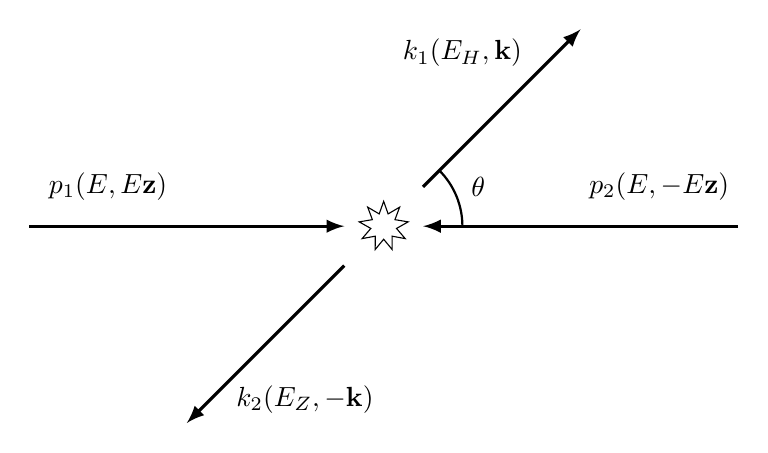
\begin{tikzpicture}[>=latex]
\draw[black,very thick,->] (0,0) -- (4,0);
\draw[black,very thick,->] (9,0) -- (5,0);
\draw[black,very thick,->] (4,-0.5) -- (2,-2.5);
\draw[black,very thick,->] (5,0.5) -- (7,2.5);
\draw[thick] (5.5,0) arc (0:45:1);
\node at(5.7,0.5){$\theta$};
\node at(1,0.5){$p_1(E,E\textbf{z})$};
\node at(8,0.5){$p_2(E,-E\textbf{z})$};
\node at(5.5,2.2){$k_1(E_H,\textbf{k})$};
\node at(3.5,-2.2){$k_2(E_Z,-\textbf{k})$};
\node at(4.5,0)[star,star points=9, star point height=0.15cm, minimum size=0.15cm, draw]{};
\end{tikzpicture}
\centering
\caption{Kinematic picture of the scattering process,}
\end{figure}\\
where $E$ denote energy of the beam, $\theta$ is the scattering angle between $e^+$ and $Z$ boson.
Our aim is to obtain the final cross-section which depends only on $E, m_Z,m_H$. Drawing and solving kinematic picture means that we are enforcing the conservation laws on the particles, thinking it as a precalculation step that help us deal with all the delta functions that lie within our scattering amplitude $\mathcal{M}$. And thus we use the conservation laws:
\begin{itemize}
\item energy
\begin{equation}
2E=E_H+E_Z
\end{equation}
\item momentum
\begin{align}
&|\textbf{k}_H|^2&&=|\textbf{k}_Z|^2 \nonumber\\
&\Rightarrow E_H^2- m_H^2&&=E_z^2-m_Z^2\nonumber\\
&\Leftrightarrow E_Z&&=E\left(1+\frac{m_Z^2-m_H^2}{4E^2}\right),\label{15}
\end{align}
\end{itemize}
thus we can deduce
\begin{equation}
E_H=E\left(1-\frac{m_Z^2-m_H^2}{4E^2}\right)\label{16},
\end{equation}
and for the momentum vector 
\begin{equation}
\begin{split}
k^2&=E_H^2-m_H^2\\
&=E^2-\frac{(m_Z+m_H^2)}{2}+\frac{(m_Z^2-m_H^2)^2}{16E^2}\\
&=E^2 \beta^2,
\end{split}
\end{equation}
with
\begin{equation}
\beta=\frac{1}{4E^2}\sqrt{\left[16E^4-8E^2(m_Z^2+m_H^2)+(m_Z^2-m_H^2)^2\right]}.
\end{equation}
We arrive at the 4-momenta of all the particles
\begin{equation}
\begin{cases}
&p_1=E(1,0,0,1)\\
&p_2=E(1,0,0,-1)\\
&k_1=E\left(1-\frac{m_Z^2-m_H^2}{4E^2},\beta \sin\theta,0,\beta \cos\theta\right)\\
&k_2=E\left(1+\frac{m_Z^2-m_H^2}{4E^2},-\beta \sin\theta,0,-\beta \cos\theta\right)\\
&q=p_1+p_2=E(2,0,0,0).
\end{cases}
\end{equation}
	Now we need to compute the dot products of various 4-vectors
\begin{align*}
&p_1.p_1=p_2.p_2=m_e^2 & &k_1.k_1=m_H^2 & &k_2.k_2=m_Z^2\\
&p_1.p_2=2E^2	 &	&q.q=(p_1+p_2)^2=4E^2 &  &p_1.q=p_2.q=2E^2	\\
&k_2.q =2EE_z & &k_2.p1=EE_Z-Ek\cos\theta &&k_2.p_2=EE_Z+Ek\cos\theta,
\end{align*}
putting all the conditions into a replace list called $Onshell$, onshell also means depends only in incoming and out going particles, not propagator
\begin{align*}
\text{onShell}=&\{\text{p1}.\text{p2}\to 2 \text{E0}^2,q.q\to 4 \text{E0}^2,\text{p1}.q\to 2 \text{E0}^2,\text{p2}.q\to 2 \text{E0}^2\\
&,\text{p1}.\text{p1}\to 0,\text{p2}.\text{p2}\to 0,\text{k2}.q\to 2 \text{E0}\ \text{Ez},\text{k2}.\text{p1}\to \text{E0}\ \text{Ez}-\text{CT}\ \text{E0} \text{k}\\
&,\text{k2}.\text{p2}\to \text{CT}\ \text{E0} \text{k}+\text{E0}\ \text{Ez},\text{k2}.\text{k2}\to \text{mz}^2\};
\end{align*}
with $E0 \equiv $E and CT$ \equiv \cos\theta_w$,
we would like to set the mass of electron equal to 0, substitute $E_Z$ and $E_H$ with \eqref{15} and \eqref{16} by making a new replacement list though the command
\begin{equation}
\text{con1}=\left\{\text{me}\to 0,\text{Ez}\to \text{E0} \left(\frac{\text{mz}^2-\text{mh}^2}{4 \text{E0}^2}+1\right)\right\};,
\end{equation}
applying the $onShell$ and $con1$ condition to \textbf{X} with the command
\begin{equation}
\text{Simplify}[X\text{/.}\, \text{onShell}\text{/.}\, \text{con1}],
\end{equation}
the out put is what wee needed for the squared amplitude
\begin{equation}
\begin{split}
\textbf{X}&=\frac{(g_A^2+g_V^2)}{2 m_Z^2} [16 E^4-8 E^2 (2 \cos^2\theta k^2+m_H^2-3 m_Z^2)+(m_H^2-m_Z^2)^2]\\
&=\frac{(g_A^2+g_V^2)}{2 m_Z^2}\left[16k^2E^2-16E^2k^2\cos^2\theta+32E^2 m_Z^2\right] .
\end{split}
\end{equation}
\subsection{analytical calculation}
\label{analytical}
We are going to evaluate this cross section in another style, not involving much computations nor tracing technique. We will write down explixit expressions for $v(p_1),u(p_2),\epsilon_\mu$. Starting with 4-momentum of $Z$ boson at rest frame
\begin{equation}
k_2=(m_Z,0,0,0),
\end{equation}
with the polarization vectors
\begin{align}
\epsilon^1_\mu=(0,1,0,0),\\
\epsilon^1_\mu=(0,0,1,0),\\
\epsilon^1_\mu=(0,0,0,1),\\
\end{align}
bosting the in the $z$ direction with transformation matrix
\begin{equation}
\Lambda^{03}=\begin{pmatrix}
cosh(\chi)&0&0&sinh(\chi)\\
0&1&0&0\\
0&0&1&0\\
sinh(\chi)&0&0&cosh(\chi)
\end{pmatrix}\quad =\quad\frac{1}{m_z}
\begin{pmatrix}
E_Z&0&0&k\\
0&1&0&0\\
0&0&1&0\\
k&0&0&E_Z
\end{pmatrix},
\end{equation}
with $E_Z^2-k^2=m_Z^2$, we then have
\begin{align}
k_2&=(E,0,0,k),\nn\\
\epsilon^1_\mu&=(0,1,0,0),\nn\\
\epsilon^2_\mu&=(0,0,1,0),\nn\\
\epsilon^3_\mu&=\frac{1}{m_Z}(p,0,0,E).
\end{align}
Last step is to spin them around the $x$ axis with
\begin{equation}
\Lambda^{23}=\begin{pmatrix}
1&0&0&1\\
0&1&0&0\\
0&0&\cos(\theta)&-\sin(\theta)\\
0&0&\sin(\theta)&\cos(\theta)
\end{pmatrix},
\end{equation}
which return us with
\begin{align}\label{aa}
k_2&=(E,0,-k \sin(\theta),k \cos(\theta))\nn\\
\epsilon^1_\mu&=(0,1,0,0),\nn\\
\epsilon^2_\mu&=(0,0,\cos(\theta),\sin(\theta)),\nn\\
\epsilon^3_\mu&=\frac{1}{m_Z}(p,0,-E\sin(\theta),E \cos(\theta)).
\end{align}
The 4-momentum and polarization vectors remain orthogonal throughout the transformations, which is the requirement for vector fields.
For our fermion fields, we have
\begin{align}
&v^s(p_1)=\begin{pmatrix}
\sqrt{p_1\cdot \sigma}\eta^s\\
-\sqrt{p_1\cdot \overline{\sigma}}\eta^s\\
\end{pmatrix} &\text{and} &&u^r(p_2)=\begin{pmatrix}
\sqrt{p_2\cdot \sigma}\xi^r \\
\sqrt{p_2\cdot \overline{\sigma}}\xi^r\\
\end{pmatrix},
\end{align}
To be more explicit:
\begin{align}
v^1(p_1)&=\sqrt{2E}\begin{pmatrix}
0&0&-1&0
\end{pmatrix}^T,
&&v^2(p_1)=\sqrt{2E}\begin{pmatrix}
0&1&0&0
\end{pmatrix}^T,\nn\\
u^1(p_1)&=\sqrt{2E}\begin{pmatrix}
1&0&0&0
\end{pmatrix}^T,
&&u^2(p_1)=\sqrt{2E}\begin{pmatrix}
0&0&0&1
\end{pmatrix}^T,
\end{align}
here we have used $p_1=(E,0,0,E)$, $p_1=(E,0,0,-E)$ $\eta^s$ and $\xi^s$ are 2-component spinors, which denote spin components. In this case, we will choose the spin basis in the $z$ direction, which translates to
\begin{align}
\eta^1=\begin{pmatrix}
1\\0
\end{pmatrix},&&\eta^2=\begin{pmatrix}
0\\1
\end{pmatrix},&&\xi^1=\begin{pmatrix}
1\\0
\end{pmatrix},&&\xi^2=\begin{pmatrix}
0\\1
\end{pmatrix}.
\end{align}
Back to our amplitude \eqref{amplitude1}
\begin{align}
\mathcal{M}=\lambda \overline{v}(p_1)\gamma^\mu (g_V-g_A\gamma^5) u(p_2) \left(g_{\mu \nu}-\frac{q_\mu q_\nu}{m_Z^2}\right) g^{\nu \rho}\epsilon_\rho^*(k_2),
\end{align}
Assuming that vector current conserved, i.e. $\partial_\mu J^\mu=0$, or in the momentum space, $q_\mu J^\mu=0$, with the vector currents is $\overline{\psi}\gamma^\mu\psi$. Writing $\mathcal{M}$ in explicit polarization and spin notations:
\begin{align}\label{ac}
\mathcal{M}&=\lambda\ \overline{v}^s(p_1)\gamma^\mu (g_V-g_A \gamma^5) u^r(p_2)  \epsilon_\mu^*(k_2)\nn\\
&=\lambda \epsilon^{i*}_\mu(k_2) \mathcal{M}^\mu(s,r),
\end{align}
here we have split the amplitude into 2 factor, $\epsilon$ is polarization, $\lambda$ is coupling constant, $\mathcal{M}^\mu$ is the rest of the amplitude.
\begin{equation}
\mathcal{M}^\mu(s,r)=\overline{v}^s(p_1)\gamma^\mu (g_V-g_A \gamma^5) u^r(p_2) .
\end{equation}
Replace all of what we have above to $\mathcal{M}^\mu(s,r)$:
\begin{align}\label{ab}
\mathcal{M}^\mu(1,1)&=0\nn\\
\mathcal{M}^\mu(2,2)&=0\nn\\
\mathcal{M}^\mu(1,2)&=2E(0\quad 0\quad-1\quad0)\gamma^0\gamma^\mu(g_V-g_A\gamma^5) \begin{pmatrix}
0\\0\\0\\1
\end{pmatrix}=-(g_V-g_A)2E(0,1,i,0)\nn\\
\mathcal{M}^\mu(2,1)&=2E(0\quad 1\quad 0\quad 0)\gamma^0\gamma^\mu(g_V-g_A\gamma^5) \begin{pmatrix}
1\\0\\0\\0
\end{pmatrix}=(g_V+g_A)2E(0,1,-i,0).
\end{align}
Substitute \eqref{aa}, \eqref{ab} into \eqref{ac}, square the amplitude then sum over all spin states and polarization state
\begin{align}
|\mathcal{M}|^2&=\frac{1}{4}\sum_{s,r}^2|\lambda \epsilon^{i*}_\mu \mathcal{M}^\mu(s,r)|^2\nn\\
&=\frac{1}{4}|\lambda|^2\left(| \epsilon^{i*}_\mu \mathcal{M}^\mu(1,2)|^2+|\epsilon^{i*}_\mu\mathcal{M}^\mu(2,1)|^2\right)\nn\\
&= 2(g_A^2+g_V^2)E^2|\lambda|^2 \left[1+\cos^2(\theta)+\frac{E^2 \sin^2(\theta)}{m_Z^2}\right]\nn\\
&=2 (g_A^2+g_V^2)E^2|\lambda|^2 \left(2+\frac{k^2 \sin^2(\theta)}{m_Z^2}\right),
\end{align}
and we have arrived at our result on previous section. We were able to do this kind of analyzing because our form of amplitude is quite simple, in more complicated amplitude, computer is the only way to go.
\section{differential and total cross-section}
The general scattering cross-section for 2 incoming particle and $n$ outcoming particle is the \textbf{\textit{Golden Rules for Scattering}} 
\begin{equation}
d\sigma=\frac{d\Pi_n}{2E_A2E_B|v_A^z-v_B^z|}.\frac{1}{4}\sum_{spin} \sum_{pol} |\mathcal{M}|^2,\label{18}
\end{equation}
where $A,B$ are incoming particles,
\begin{equation}
|v_A^z-v_B^z|=|\frac{\textbf{p}_1}{E}-\frac{\textbf{p}_2}{E}|=2,
\end{equation}
$d\Pi_n$ is the phase space integral for n-body scattering 
\begin{equation}
d\Pi_n=\int \left(\prod_{f=1}^n\frac{d^3\textbf{p}_f}{(2\pi)^3 2E_f}\right)(2\pi)^4\delta^{(4)}\left(p_A+p_b-\sum p_f\right),
\end{equation}
here $f$ count all the out going particles and the delta function enforce the conservation laws, for 2 particles in the final state we have
\begin{equation}
d\Pi_2=\int \left(\frac{d^3\textbf{k}_1}{(2\pi)^3 2E_H}\frac{d^3\textbf{k}_2}{(2\pi)^3 2E_Z}\right)(2\pi)^4\delta^{(4)}\left(p_1+p_2-k_1-k_2\right).
\end{equation}
Since $\textbf{p}_1+\textbf{p}_2=0$ (in the CM frame), we can integrate over $\textbf{k}_1$ by setting
$\textbf{k}_1=-\textbf{k}_2=\textbf{k}$ , leaving us left with the remaining triple integral
\begin{align}
d\Pi_2&=\int \frac{d^3\textbf{k}_2}{(2\pi)^2 4E_Z E_H}\delta\left(2E-E_H-E_Z\right)\nonumber\\
&=\int \frac{d^3\textbf{k}_2}{(2\pi)^2 4E_Z E_H}\delta\left(2E-E_H-E_Z\right)\nonumber\\
&=\int \frac{k^2 dk d(\cos\theta) d\phi}{(2\pi)^2 4E_Z E_H}\delta\left(2E-\sqrt{m_H^2+k^2}-\sqrt{m_Z^2+k^2}\right)\nonumber\\
\Rightarrow \frac{d\Pi_2}{d(cos\theta)}&=\int \frac{k^2 dk}{(2\pi) 4E_Z E_H}\delta\left(2E-\sqrt{m_H^2+k^2}-\sqrt{m_Z^2+k^2}\right)\nonumber\\
&=\int \frac{k^2 dk}{(2\pi) 4E_Z E_H}\frac{\delta\left(k-k_{0}\right)}{\frac{k}{\sqrt{m_H^2+k^2}}+\frac{k}{\sqrt{m_Z^2+k^2}}}\nonumber\\
&=\int \frac{k^2 dk}{(2\pi) 4E_Z E_H}\frac{\delta\left(k-k_{0}\right)}{\frac{k}{E_H}+\frac{k}{E_Z}}\nonumber\\
&=\frac{k^2}{(2\pi) 4E_Z E_H}\frac{1}{\frac{k}{E_H}+\frac{k}{E_Z}}\nn\\
&=\frac{k}{8\pi}\frac{1}{E_H+E_Z}\nn\\
&=\frac{k}{8\pi}\frac{1}{2E},
\label{17}
\end{align}
here $k_0$ is the value of $|\textbf{k}|$ that is consistent with conservation of energy. Plugging \eqref{20} and \eqref{17} into $Golden$ $Rules$ $for$ $Scattering$ \eqref{18} 
\begin{align}
\frac{d\sigma}{d(\cos\theta)}&=\frac{1}{2E2E|v_1^z-v_2^z|}.\frac{k}{8\pi}\frac{1}{2E}.|\lambda|^2\frac{1}{4}\textbf{X}\nn\\
&=\frac{\beta}{128\pi E^2} |\lambda|^2 \frac{1}{4}\frac{(g_A^2+g_V^2)}{2 m_Z^2}\left[16k^2E^2(1-\cos^2\theta)+32E^2 m_Z^2\right] \label{23}
 ,
\end{align}
integrating over $d(\cos\theta)$and inserting $\lambda$ from $\eqref{21}$ give the total cross-section
\begin{align}
\int_{-1}^1 \frac{d\sigma}{d(\cos\theta)}= \sigma &=\frac{\beta}{128\pi E^2}. |\lambda|^2 \frac{1}{4}\frac{(g_A^2+g_V^2)}{2 m_Z^2}\left[16\pi  \frac{4}{3} k^2E^2+64m_Z^2 E^2\right]\nn\\
&=\frac{\alpha^2 \pi\beta}{4}\frac{\ m_Z^2}{ (q^2-m_Z^2)^2} \frac{ (g_A^2+g_V^2) }{s^4 _w c^4_w}\left[ \frac{E^2\beta^2}{3m_Z^2} +1\right],
\end{align}
the result has been cross checked with \cite{Denner:1992bc}\\
\begin{figure}[ht]
\centering
	\begin{picture}(100,60)
    \put(50,0){$E_{CM}$(GeV)}
    \put(-7,40){$\sigma$(fb)}
    \put(0,5){\includegraphics[scale=0.7]{SMscatter.pdf}}
    \end{picture}
\caption{Total cross-section of $e^+e^- \rightarrow ZH$ in SM, specified point will be used to plot the differential cross-section tin the next figure}
\label{fig:SMcross-section}
\end{figure}
\begin{figure}[h]
\centering
\begin{picture}(100,80)
    \put(50,0){$\theta$ (Rad)}
    \put(-7,40){$\frac{d\sigma}{\cos \theta}$(fb)}
    \put(0,5){\includegraphics[scale=0.7]{diff-cross.pdf}}
    \end{picture}
\caption{differential cross-section of $e^+e^- \rightarrow ZH$ at $E_{CM}=220,250,400$ GeV }
\label{diff-cross}
\end{figure}
We can see that cross-section in figure \ref{fig:SMcross-section} peaks at the energy that is a bit higher than $m_h+m_Z$, and falls off quite quickly, this means that production of Higgs boson from the $e^+ + e^- \rightarrow Z H$ process lies mostly at the GeV energy scale. In figure \ref{diff-cross}, contribution of $1-\cos^2 \theta$ to the differential cross section \eqref{23} began to "take shape" as the energy get higher, but dependence from all angle of scatting $\theta$ is not that significant.
\newpage
\section{Introducing the $Z'$ boson}
There are models that introduce a new gauge boson boson $Z'$ which has the same property as $Z$ boson such as Grand Unified Theories
, Superstring Theories , Left-Right Symmetric
Models , and other models such as models of
composite gauge bosons \cite{Gutierrez-Rodriguez:2015qka}. We will consider $Z'$ boson that is introduce in $B-L$ (baryon number minus lepton number) model \cite{Basso:2011hn}. Since $Z'$ is an extra gauge boson, it does has the similar couplings as $Z$ boson apart from the coupling parameter $\lambda$. Thus we proceed to write down the general Feynman rules for $Z'$ boson
\pagebreak
\begin{align}
\feynmandiagram [inline=(a.base),horizontal=a to b] {
  i1 [particle=$e^-$] -- [fermion] a -- [fermion] i2 [particle =$e^+$],
  a -- [photon] b [particle=$Z'$],
};
& &&=\lambda_{eeZ'} \times \gamma^\mu(g_V'-g_A') \gamma^5\\
\feynmandiagram [inline=(d.base),horizontal=b to d] {
a [particle=\(Z\)]  -- [boson] b -- [boson] c[particle =\(Z'\)],
b -- [scalar] d [particle=\(h\)],
};
& &&=\lambda_{ZZ'h} \times g^{\mu \nu}\\
 \feynmandiagram [inline=(a.base),medium, horizontal=a to b]{
    a [dot] -- [boson,edge label=\(Z'\) ] b [dot]
    };&=\frac{-i}{p^2-m_Z'^2+im_{Z'} \Gamma_{Z'}}\left(g_{\mu \nu}-\frac{q_\mu q_\nu}{ m^2_{Z'}}\right)&&=\lambda_{Z'Z'}\times (g_{\mu\nu}-\frac{q_\mu q_\nu}{m_{Z'}^2}),
\end{align}
here $\Gamma_{Z'}$ is the total decay width of $Z'$ boson, sum over all possible decay process, this factor is $Breit-Wigner$ parameters to negate the exploding in total cross-section at the resonance frequency, we would like to add the similar factor to our SM $Z$ boson also. The parameters $\lambda$ will be worked out in next section, we will assume they as constant for this section.
\begin{figure}
\begin{align}
&\feynmandiagram [medium, horizontal=b to d] {
a [label=$e^-$] -- [fermion] b -- [fermion] c[label=$e^+$],
b -- [boson,edge label =$Z$] d,
e[label=$Z$] -- [boson] d -- [scalar] f[label=$h$]
};,&&\quad
\feynmandiagram [medium, horizontal=b to d] {
a [label=$e^-$] -- [fermion] b -- [fermion] c[label=$e^+$],
b -- [boson,edge label =$Z'$] d,
e[label=$Z$] -- [boson] d -- [scalar] f[label=$h$]
};\nn\\
&\qquad\qquad\qquad M_1 &&\qquad\qquad\qquad M_2\nn
\end{align}
\caption{ Feynman diagram for the process $e^+e^-\rightarrow Zh$ with extra gauge boson }
\end{figure}\\

The total square amplitude is 
\begin{equation}
|\mathcal{M}|^2=|\mathcal{M}1+\mathcal{M}2|^2=|\mathcal{M}1|^2+|\mathcal{M}2|^2+2\Re( \mathcal{M}1 \mathcal{M}2^*),\label{22}
\end{equation}
$|\mathcal{M}1|^2$ is the $|\mathcal{M}|^2$ in \ref{section1} with slight change in name and we replace the denominator of Z boson with $q^2-m_Z^2+im_Z$
The amplitude for the $Z'$ contributed diagram contribution
\begin{align}
\mathcal{M}2
=&\lambda' \overline{v}(p_1)(g_V'+g_A' \gamma^5)\left(\gamma^\mu-\frac{\slashed{q}q^\mu}{m_{Z'}^2}\right) u(p_2) \epsilon^*_\mu (k_2),
\end{align}
The kinematic picture stays the same for 2 processes so we can follow the  procedure of \ref{section1} and arrive with the result
\begin{equation}
\frac{1}{4}\sum_{spin} \sum_{pol} |\mathcal{M}2|^2=|\lambda'|^2\frac{1}{4} \frac{(g_A'^2 + g_V'^2)}{2m_{Z}^2} (16E^2k^2- 16E^2k^2\cos^2 \theta  +
   32 E^2m_{Z}^2).
\end{equation}

Third term of \eqref{22},
averaging over the initial spin states and sum over the final polarizations of Z boson
\begin{equation}
\frac{1}{4}\sum_{spin} \sum_{pol}\mathcal{M}1 \mathcal{M}2^*=\frac{1}{4}\lambda \lambda'^*\frac{g_Ag_A'+g_Vg_V'}{m_Z^2}(16E^2k^2- 16E^2k^2\cos^2 \theta  +
   32 E^2m_{Z}^2).
\end{equation}
Having calculated all the needed amplitude, we can now sum them all up
\begin{align}
\frac{1}{4}\sum_{spin} \sum_{pol}\left[|\mathcal{M}|1^2+|\mathcal{M}2|^2+2\Re( \mathcal{M}1 \mathcal{M}2^*)\right]=&\frac{1}{4} (16E^2k^2- 16E^2k^2\cos^2 \theta  +32 E^2m_{Z}^2)\nn\\
\times &\left[|\lambda|^2\frac{(g_A^2 + g_V^2)}{2m_{Z}^2}+|\lambda'|^2 \frac{(g_A'^2 + g_V'^2)}{2m_{Z}^2}+2Re(\lambda \lambda'^*)\frac{g_Ag_A'+g_Vg_V'}{2m_Z^2}\right].
\end{align}
The coupling parameters $\lambda$ and $\lambda'$ need a bit work to return at their squared module because $\lambda_{ZZ}$ and $\lambda_{Z'Z'}$ have complex denominator
\begin{align}
|\lambda|^2&=|\lambda_{eeZ}\lambda_{ZZH}|^2 \frac{1}{(q^2-m_Z^2)+(m_Z\Gamma_Z)^2}\\
|\lambda'|^2&=|\lambda_{eeZ'}\lambda_{Z'ZH}|^2 \frac{1}{(q^2-m_{Z'}^2)+(m_{Z'}\Gamma_{Z'})^2}\\
Re(\lambda\lambda'^*)&=\lambda_{eeZ} \lambda_{ZZH}\lambda_{eeZ'}^* \lambda_{Z'ZH}^* \nn\\
&\times \frac{\left[(q^2-m_Z^2)(q^2-m_{Z'}^2)+m_Z\Gamma_Zm_{Z'}\Gamma_{Z'}\right] }{\left[(q^2-m_Z^2)(q^2-m_{Z'}^2)+m_Z\Gamma_Zm_{Z'}\Gamma_{Z'}\right]^2+\left[(q^2-m_Z^2)m_{Z'}\Gamma_{Z'}-(q^2-m_{Z'}^2)m_Z\Gamma_Z\right]^2}.
\end{align}
The phase space integral remains the same so we can plug $|\mathcal{M}|^2$ into \eqref{18} for the cross-section
\begin{align}
\frac{d\sigma}{d(\cos\theta)}=&\frac{d\Pi_n}{2E_A2E_B|v_A^z-v_B^z|}.\frac{1}{4}\sum_{spin} \sum_{pol} |\mathcal{M}|^2\\
=&\frac{\beta}{512\pi E^2}(16E^2k^2- 16E^2k^2\cos^2 \theta  +32 E^2m_{Z}^2)\nn\\
\times& \left[|\lambda|^2\frac{(g_A^2 + g_V^2)}{2m_{Z}^2}+|\lambda'|^2 \frac{(g_A'^2 + g_V'^2)}{2m_{Z}^2}+2Re(\lambda \lambda'^*)\frac{g_Ag_A'+g_Vg_V'}{2m_Z^2}\right],
\end{align}
integrating $d(cos\theta)$ yields
\begin{align}
\sigma=&\frac{\beta}{512\pi E^2}\left(16  \frac{4}{3} k^2E^2+64m_Z^2 E^2\right)\nn\\
&\times \left[|\lambda|^2\frac{(g_A^2 + g_V^2)}{2m_{Z}^2}+|\lambda'|^2 \frac{(g_A'^2 + g_V'^2)}{2m_{Z}^2}+2Re(\lambda \lambda'^*)\frac{g_Ag_A'+g_Vg_V'}{2m_Z^2}\right]\\
=&\frac{\beta m_Z^2}{8\pi}\left(\frac{\beta^2 E^2}{3 m_Z^2}+ 1\right)\nn\\
&\times \left[|\lambda|^2\frac{(g_A^2 + g_V^2)}{2m_{Z}^2}+|\lambda'|^2 \frac{(g_A'^2 + g_V'^2)}{2m_{Z}^2}+2Re(\lambda \lambda'^*)\frac{g_Ag_A'+g_Vg_V'}{2m_Z^2}\right].
\end{align}
\section{The Baryon number minus Lepton number model}
Anomaly plays a important role on deciding if a quantum theory is consistent or not, Standard Model has nicely cancel out all the anomalies and there it is still standing today. But there is still a room for an extra $U(1)$ force acting on the model which have the following $Y'$ charges
\begin{equation}
    Y'_L=Y'_{e_R}=Y'_{\nu_R}=-1, \quad  Y'_Q=Y'_{u_R}=Y'_{d_R}=\frac{1}{3},
\end{equation}
these charges are exactly like the baryon minus lepton number, so this new group is called $U(1)_{B-L}$.
In this section we briefly introduce the Baryon number minus Lepton number model ($B-L$) as a minimal extension of SM. It is minimal in the sense that it is a modification to our SM, we mannually add many of new factors in the SM lagrangian . Our SM covariant takes an extra $U(1)$ factor from the new symmetry group. In  the Higgs sector, an extra scalar singlet is added in the Higgs Lagrangian to spontaneously break the new $U(1)$ factor. An extra right-handed neutrino term is added in the fermion sector which mass is given by the new scalar field, and cancel out the anomalies \cite{Basso:2011hn}.
\subsection{Covariant derivative}
Covariant derivative for $B-L$ model is
\begin{align}
D_\mu=\partial_\mu - ig_s \frac{\lambda^a}{2}G_\mu^a-i g I_a W_\mu^a-i g' YB_\mu -i(\tilde{g} Y+ g_1' Y_{B-L})B_\mu',
\end{align}
where $Y_{B-L}$ is simply baryon minus lepton number, i.e, $-1$ for lepton and $1/3$ for quarks with no distinction between generations. $\tilde{g},g_1'$ are free parameters, by alter them we can fix the model to some of the popular $Z'$ models. In $pure$ $B-L$ model, $\tilde{g}$ takes the value 0, that means there is no mixing between $Z$ and $Z'$. The mixing occurs at a very small angle to study phenomenons of the extra $U(1)$ factor and for the $Z'$ boson.\\
\subsection{Fermion Lagrangian}
The fermion Lagragian is
\begin{align}
\mathcal{L}_{fermion}=& i\overline{L}(x) \gamma^\mu D_\mu L(x)+i\overline{Q}_L(x) \gamma^\mu D_\mu Q_L(x)+
i\overline{e}_R(x) \gamma^\mu D_\mu e_R(x)\nn\\+
&i\overline{u}_R(x) \gamma^\mu D_\mu u_R(x)+
i\overline{d}_R(x) \gamma^\mu D_\mu d_R(x)+
i\overline{\nu}_R(x) \gamma^\mu D_\mu \nu_R(x),
\end{align}
sum over all 3 fermions generations. The Lagrangian stays pretty much the same as in SM case, we have introduced the right-handed neutrino but we do not discuss about that in this thesis.
\subsection{Yang-Mills Lagrangian}
The Yang-mills Lagrangian gets an extra strength tensor for the added $B'_\mu$ field
\begin{equation}
\mathcal{L}_{gauge}= 
-\frac{1}{4}W_{\mu\nu}^iW^{\mu\nu}_i-\frac{1}{4}G_{\mu\nu}^iG^{\mu\nu}_i-\frac{1}{4}B_{\mu\nu}B^{\mu\nu}-\frac{1}{4}B_{\mu\nu}'B^{'\mu\nu }
\end{equation}
where
\begin{equation}
B'_{\mu\nu}=\partial_\mu B'_\nu -\partial_\nu B'_\mu
\end{equation}
\subsection{Yukawa Lagrangian}
The Yukawa interactions are
\begin{equation}
\begin{split}
\mathcal{L}_Y=&-G_l^{ij}\overline{L}^{i}_L\phi l^{j}_R -G_d^{ij}\overline{Q}^{i}_L\phi d_R^{j}-G_u^{ij}\overline{Q}^{i}_L\phi^c u_R^{j}\\
&-G^{ij}_\nu\overline{L}^{i}_L \phi^c \nu_R^{j}-G_M\overline{\nu_R^c}^{i}\chi\nu_R^{j}+h.c,
\end{split}
\end{equation}
here the superscripts $i,j=[1,2,3]$ are generation indices, and $\phi=(0\ v)^T$, $\phi^c=i\sigma^2\phi$
\subsection{Higgs Lagrangian and spontaneous symmetry breaking}
To give mass to the extra neutral gauge field associated to the new $U(1)$ factor, we only need one extra degree of freedom, the most efficient way to do this is to add a new scalar singlet. The singlet is required to acquire vacuum expectation value at the TeV scale.
The Higgs Lagrangian is
\begin{equation}
\mathcal{L}_{higgs}=(D^\mu H)^\dagger D_\mu H+(D^\mu\chi)^\dagger  D_\mu \chi- V(H,\chi) \label{kinetic B-L},
\end{equation}
with the potential
\begin{align}
V(H,\chi)=& m^2H^\dagger H+\mu^2|\chi|^2+\begin{pmatrix}
H^\dagger H & |\chi|^2
\end{pmatrix}
\begin{pmatrix}
\lambda_1 & \frac{\lambda_3}{2}\\
\frac{\lambda_3}{2}& \lambda_2
\end{pmatrix}
\begin{pmatrix}
H^\dagger H\\
|\chi|^2
\end{pmatrix}\nn\\
=&m^2 H^\dagger H+\mu^2|\chi|^2+ \lambda_1(H^\dagger H)^2+\lambda_2 |\chi|^4+\lambda_3 H^\dagger H|\chi|^2\label{protential'},
\end{align}
where $H$ and $\chi$ are complex scalar Higgs doublet and singlet respectively. For the $B-L$ charges, $\chi$ takes the value $+2$, $H$ takes the value 0 to ensure gauge invariant of the fermion sector \cite{Basso:2011hn}.
The minimum configuration of the potential \eqref{protential'} is where the fields at the state that satisfy the condition $H_0^\dagger H_0=v^2/2$ and $|\chi_0|^2=x^2/2$, with the explicit $VEV$'s is
\begin{align}
x^2&=2\frac{\lambda_3 \mu^2-2\lambda_1 m^2}{4\lambda_1 \lambda_2-\lambda_3^2}\label{scalar1}\\
v^2&=2\frac{\lambda_3 \mu^2- 2\lambda_2 m^2}{4 \lambda_1 \lambda_2- \lambda_3^2}\label{scalar2},
\end{align}
where $x^2$ and $v^2$ both have to be positive, in term of conditions for the parameters we have:
\begin{equation}
\begin{cases}
&\lambda_2 m^2<\frac{\lambda_3}{2}\mu^2\\
&\lambda_1 \mu^2<\frac{\lambda_3}{2}m^2.
\end{cases}
\end{equation}
 We will chose a real and electrically neutral state the scalar fields analogous to the SM in the form 
\begin{align}
\langle H_0 \rangle =\frac{1}{\sqrt{2}}\begin{pmatrix}
0\\ v
\end{pmatrix},&& \langle \chi_0 \rangle =\frac{x}{\sqrt{2}},
\end{align}
expanding them around the minima of their vacuum
\begin{align}
H=\frac{1}{\sqrt{2}}\begin{pmatrix}
w_1+ iw_2\\
v +h + i z
\end{pmatrix},&&\chi=\frac{1}{\sqrt{2}}(x+[h'+iz')] .
\end{align}
where $w^\pm=w_1\mp iw_2$, $z$ and $z'$ are the Goldstone which will be absorbed to give mass to $W^\pm$, $Z$ and $Z'$, respectively. Using freedom of phase transformation to eliminate all the Goldstone bosons leave us with the Higgs fields :
\begin{align}
H=\frac{1}{\sqrt{2}}\begin{pmatrix}
0\\
v +h
\end{pmatrix},&&\chi=\frac{1}{\sqrt{2}}(x+h') .
\end{align}

Since we are studying the extension of the Abelian gauge group, the non-Abelian related only components like $W^1_\mu$ and $W^2_\mu$ stay unchanged. Expand the scalar kinetic term in \eqref{kinetic B-L} yields
\begin{align}
 (D^\mu H)^\dagger D_\mu H&=\frac{1}{2}\partial_\mu h \partial^\mu h+\frac{1}{8} \begin{pmatrix}
 0 &v+h
 \end{pmatrix} ( g\sigma_a W_\mu^a+g' B_\mu+  \tilde{g} B_\mu')\begin{pmatrix}
 0\\v+h
 \end{pmatrix}\nn\\
 &=\frac{1}{2}\partial_\mu h \partial^\mu h+ \frac{1}{8}(v+h)^2\left[g(W_\mu^1)^2+ g(W_\mu^2)^2+ (-gW_\mu^3+g' B_\mu +\tilde{g}B_\mu'\right)^2]\label{Higgskin}
 \end{align} 
and
\begin{equation}
 (D^\mu\chi)^\dagger D_\mu\chi=\frac{1}{2}\partial_\mu h' \partial^\mu h'+\frac{1}{2}(x+h)^2(g_1' 2 B_\mu')^2\label{Higgskin2},
\end{equation}
we can see that the charged gauge bosons $W^\pm$ remain the same as in SM. Other neutral gauge bosons $ W_3^\mu$, $ B_\mu$, $B_\mu'$  do not have diagonalized mass so we have to introduce mass eigenstates fields that are  linear combination of them . As for the mass matrix, it takes  the form
\begin{align}
\frac{1}{2}\left(\frac{v}{2}\right)^2 \begin{pmatrix}
W^3& B_\mu & B'_\mu
\end{pmatrix}\begin{pmatrix}
g^2& -g g'& -g \tilde{g}\\
-g g'&g'^2& g' \tilde{g}\\
-g \tilde{g}& g' \tilde{g} &\tilde{g}^2+ 16 g_1'^2\left(\frac{x}{v}\right)^2
\end{pmatrix}\begin{pmatrix}
W^3\\ B_\mu \\ B'_\mu
\end{pmatrix},
\end{align}
the mass eigenvalues of the new physical fields then are:
\begin{align}
m^2_A=&0,\\
m^2_Z=&\frac{v^2}{8}\left[g^2+g'^2+16 g_1'^2 x^2/v^2+\tilde{g}^2\right.\nn\\ 
&\left.-\sqrt{\left(g^2+{g'}^2+16 {g'}^2 {x^2/v^2}+{\tilde{g}}^2\right)^2+4 \left(-16 g^2 {g_1'}^2 {x^2/v^2}-16 {g'}^2 {g_1'}^2 {x^2/v^2}\right)}\right]\\
m^2_{Z'}=&\frac{v^2}{8}\left[ g^2+{g'}^2+16 {g_1'}^2 {x^2/v^2}+{\tilde{g}}^2\right.,\nn\\
&+\left.\sqrt{\left(g^2+{g'}^2+16 {g'}^2 {x^2/v^2}+{\tilde{g}}^2\right)^2+4 \left(-16 g^2 {g_1'}^2 {x^2/v^2}-16 {g'}^2 {g_1'}^2 {x^2/v^2}\right)}\right],
\end{align}
the change of basis from the symmetry eigenstate to mass eigenstate is 
\begin{equation}
\begin{pmatrix}
B_\mu\\ W_\mu^3\\ B_\mu'
\end{pmatrix}=\begin{pmatrix}
\sin \theta_w & \cos \theta_w \cos \phi_{BL} & -\cos\theta_w  \sin\phi_{BL}\\
\cos \theta_w & -\sin \theta_w \cos \phi_{BL} & \sin\theta_w  \sin\phi_{BL}\\
0& \sin\phi_{BL}& \cos\phi_{BL}
\end{pmatrix}\begin{pmatrix}
A_\mu\\ Z_\mu\\Z'_\mu
\end{pmatrix}\label{transformmatrix},
\end{equation}
with $-\pi/4 \leqslant \phi_{BL} \leqslant \pi/4$ and 
\begin{equation}
\tan(2\phi_{BL})=\frac{2\tilde{g}\sqrt{g^2+g'^2}}{\tilde{g}^2 +16 (x/v)^2 g_1'^2-g^2-g_1^2},\label{mixingangle}
\end{equation}
In pure $B-L$ model, that is $\tilde{g}=0$, the mixing angle vanish, hence no mixing occurs, the $Z$ boson is exact our SM $Z$ boson and their masses are :
\begin{equation}
\begin{cases}
m_Z&=\frac{v}{2}\sqrt{g^2+g'^2}\\
m_{Z'}&=2 g_1' x
\end{cases}
\end{equation}

Another mixed eigenstates are Higgs fields masses in \eqref{scalar1} and \eqref{scalar2}. After the calculation, the mass of the 2 Higgs fields are:
\begin{align}
m_{h_1}^2=\lambda_1 v^2+\lambda_2 x^2-\sqrt{(\lambda_1 v^2-\lambda_2 x^2)^2+(\lambda_3 x v)^2}\\
m_{h_2}^2=\lambda_1 v^2+\lambda_2 x^2+\sqrt{(\lambda_1 v^2-\lambda_2 x^2)^2+(\lambda_3 x v)^2},
\end{align}
change of basis is
\begin{equation}
\begin{pmatrix}
h_1\\ h_2
\end{pmatrix}=\begin{pmatrix}
\cos \alpha & -\sin \alpha\\
\sin \alpha & \cos \alpha,
\end{pmatrix}\begin{pmatrix}
h\\ h'
\end{pmatrix},\label{higgsmix}
\end{equation}
with
\begin{align}
\sin 2\alpha=\frac{\lambda_3 x v}{\sqrt{(\lambda_1 v^2- \lambda_2 x^2)^2+(\lambda_3 x v)^2}},
\end{align}
if the mixing angle happens to be 0 then $h_1$ is purely our SM Higgs boson. In this thesis, we will treat $h_1$ as our SM Higgs boson and its mass is $125.1$ (GeV). We are freely to chose the mixing angle because all the $\lambda$ parameters are currently unknown and the $h'$ boson doesn't couple to normal matters like $h$ boson does, so the only boson that could interact with SM matters should be $h_1$.
\section{Few example couplings}
Here will set $\tilde{g} Y+g_1' Y_{B-L}=g_1' Y^E$ as effective coupling, with $Y^E(fermion)=1,Y^E(\chi)=2,Y^E(H)=1/2$ for all fermions,it would be in fact be different but we just want to observe the behavior of the $Z'$ boson so this approximation is good enough, the mixing angle at the value $\phi_{BL}=10^{-3}$.
\subsection{$Z'-\overline{f}-f$ vertex}
Similar to the previous chapter, expanding the fermion Lagrangian yields the fermion couplings to gauge bosons
\begin{align}
\overline{\psi}(x) \gamma^\mu D_\mu \psi(x)\subset \
 \overline{\psi}(x) \gamma^\mu &[g T_3 W_\mu ^3+g' Y B_\mu+ (g_1'  Y+ g_1' Y_{B-L})B_\mu'] \psi(x)\nn\\
 = \overline{\psi}(x)\gamma^\mu \bigg\{ &\left[g c_bc_w T_3-g' c_b s_w Y+g_1'  s_bY+g_1' s_b Y_{B-L}\right] Z_\mu \nn\\
 +&\left[-g s_bc_w T_3+g' s_b s_w Y+g_1'  c_bY+g_1' c_b Y_{B-L}\right] Z'_\mu \nn\\
 +&\left[g s_w T_3+ c_w g' Y\right]A_\mu\bigg\}
  \psi(x)\label{Z'int},
\end{align}
insert left-handed and right-handed fermion fields into \eqref{Z'int} yields the coupling between bosons and pair of fermion fields:
\begin{equation}
\mathcal{L}_{NC}=\frac{ig}{2c_w} \overline{f} \gamma^\mu(g_V-g_A \gamma^5) Z_\mu f+\frac{ig}{2c_w} \overline{f} \gamma^\mu(g_V'-g_A' \gamma^5) Z'_\mu f,
\end{equation}
where
\begin{align}
g_V&=T_3 \cos\phi_{BL}-2Q\sin^2 \theta_w \cos \phi_{BL}+\frac{2  g_1'}{g}Y^E\cos\phi_{BL}\sin\theta_w,\\
g_A&=T_3\cos \phi_{BL},\\
g_V'&=-T_3 \sin\phi_{BL}+2Q\sin^2 \theta_w \sin \phi_{BL}+\frac{2  g_1'}{g}Y^E\cos\phi_{BL}\cos\theta_w,\\
g_A'&=-T_3\sin \phi_{BL}.
\end{align}
\subsection{$Z-Z'-H$ vertex}
Expand Higgs kinetic terms \eqref{Higgskin} and \eqref{Higgskin2} by using transformation in \eqref{transformmatrix} yields us the interaction Lagrangian
\begin{align}
 (D^\mu H)^\dagger D_\mu H&\subset - \frac{v}{4}\left[\frac{4g_1' m_Z}{v}\cos 2\phi_{BL}+\left(\frac{4m^2_Z}{v^2} -g_1'^2\right)\sin 2\phi_{BL}\right] hZ_\mu Z_\mu'\\
  (D^\mu\chi)^\dagger D_\mu\chi &\subset  4 g_1'^2 \sin (2\phi_{BL}) x  \ h' Z_\mu Z_\mu'.
\end{align}
Apply the Higgs mixing in \eqref{higgsmix} and pull out the terms that involve $h_1,Z_\mu,Z_\mu'$
\begin{align}
\mathcal{L}_{hZZ'}=&\frac{v}{4} \big[f(\phi_{BL})\cos \alpha-g(\phi_{BL}) \sin \alpha\big] \ h_1 Z_\mu Z_\mu',
\end{align}
with
\begin{align}
f(\phi_{BL})&=\frac{4g_1'  m_Z}{v}\cos 2\phi_{BL}+\left(\frac{4m^2_Z}{v^2} -g_1'^2\right)\sin 2\phi_{BL},\\
g(\phi_{BL})&= 16 g_1'^2 \frac{x}{v}\sin (2\phi_{BL}),
\end{align}
take note that we consider $h_1$ as our SM Higgs boson. 
\section{Decay width of $Z'$}
A pretty useful way of calculate the magnitudes of the out going momenta of the decaying process $(1\rightarrow 2+3)$ where particle 1 is at rest
\begin{align}
|\textbf{p}_2|=|\textbf{p}_3|=\frac{\sqrt{\lambda(m_1^2,m_2^2,m_3^2)}}{2m_1},
\end{align}
with
\begin{equation}
\lambda(x,y,z)=x^2+y^2+z^2-2xy-2xz-2yz,
\end{equation}
which is the so-called $triangle\ function$.

Analogue to the previous section, we will denote our $\beta$ function as
\begin{equation}
|\textbf{p}_2|=|\textbf{p}_3|=\frac{m_1}{2}\beta=\frac{m_1}{2}\sqrt{\lambda\left(1,\frac{m_2^2}{m_1^2},\frac{m_3^2}{m_1^2}\right)}.
\end{equation}
We shall calculate the decay width of $Z'$ boson, we only work out a couple of signature 2-body decay modes that is dominant contributions  the total width to evaluate our cross-section.


\subsection{Decay to $Z,h$}
\begin{equation}
\feynmandiagram [medium, horizontal=b to d] {
b[label=$Z'$] -- [boson,momentum=$p_1$] d,
e[label=$Z$] -- [boson,rmomentum'=$p_2$] d -- [scalar,momentum=$p_3$] f[label=$h$]
};\nn
\end{equation}
Feynman amplitude for $(Z'\rightarrow Zh)$ is
\begin{align}
\mathcal{M}&=\lambda_{ZZ'h} \epsilon_\mu^*(p_1)g^{\mu\nu} \epsilon_\nu^*(p_2)
\end{align}
\begin{align}
\Rightarrow \frac{1}{3}\sum_{pol}|\mathcal{M}|^2&=\frac{1}{3}|\lambda_{ZZ'h}|^2 \left(-g_{\mu \nu}+\frac{p_{1\mu}p_{1\nu}}{m_Z^2}\right)\left(-g^{\mu \nu}+\frac{p^{2\mu}p^{2\nu}}{m_{Z'}^2}\right)\nn\\
&=\frac{1}{3}|\lambda_{ZZ'h}|^2\left(3+\frac{\beta^2 m_{Z'}^2}{4m_Z^2}\right),
\end{align}
apply the \textit{Golden Rule for Decaying}
\begin{align}
\Gamma(Z'\rightarrow ZH)&=\frac{|\textbf{p}_2|}{8 \pi m_{Z'}^2}\frac{1}{3}\sum_{pol}|\mathcal{M}|^2\nn\\
&=\frac{\beta}{192 \pi m_{Z'}}|\lambda_{ZZ'h}|^2\left(12+\frac{\beta^2 m_{Z'}^2}{m_Z^2}\right)\nn\\
&=\frac{\beta}{768\pi}\frac{ c_w^2 m_{Z'}}{g^2 }\left(\frac{12 m_{Z}^2}{m_{Z'}^2}+\beta^2\right)\left[f(\theta)\cos \alpha- g(\theta)\sin \alpha\right]^2.
\end{align}
\subsection{Decay to fermions}
\begin{equation}
\feynmandiagram [medium, horizontal=b to d] {
b[label=$Z'$] -- [boson,momentum=$p_1$] d,
e[label=$\overline{f}$] -- [fermion,rmomentum'=$p_3$] d -- [fermion,momentum=$p_2$] f[label=$f$]
};\nn
\end{equation}
Feynman amplitude for $(Z'\rightarrow ff)$ is
\begin{align}
\mathcal{M}&=\overline{u}(p_2) \lambda_{ffZ'}\gamma^\mu(g_V'-g_A' \gamma^5) v(p_3) \epsilon_\mu(p_1),
\end{align}
\begin{align}
\Rightarrow\frac{1}{3}\sum_{spin}\sum_{pol}|\mathcal{M}|^2=&\frac{1}{3}N_c |\lambda_{ffZ'}|^2Tr\left[(\slashed{p}_2+m_f) \gamma^\nu(g_V'-g_A' \gamma^5)\right.\nn\\
&\times \left.(\slashed{p}_3-m_f) \gamma^\nu(g_V'-g_A' \gamma^5)\right]\left(-g_{\mu\nu}+\frac{p_{1\mu}p_{1\nu}}{m_{Z'}^2}\right)\nn\\
=&\frac{4}{3}N_c |\lambda_{ffZ'}|^2\left[g_A'^2(m_{Z'}^2-4m_f^2)+g_V'^2(m_{Z'}^2+2m_f^2)\right]
\end{align}
where $N_c$ is the number of fermion color. Apply the \textit{Golden Rule for Decaying}
\begin{align}
\Gamma(Z'\rightarrow ff)&=\frac{|\textbf{p}_2|}{8 \pi m_{Z'}^2}\frac{1}{3}\sum_{pol}\sum_{spin}|\mathcal{M}|^2\nn\\
&=\frac{\beta}{12 \pi m_{Z'}} N_c |\lambda_{ffZ'}|^2[g_A'^2(m_{Z'}^2-4m_f^2)+g_V'^2(m_{Z'}^2+2m_f^2],\label{24}
\end{align}
total decay width will be summed over all 3 generations of fermions.
\subsection{Decay to $W^{\pm}$}
\begin{equation}
\feynmandiagram [medium, horizontal=b to d] {
b[label=$Z'_\mu$] -- [boson,momentum=$p_1$] d,
e[label=$W^+_\nu$] -- [boson,rmomentum'=$p_2$] d -- [boson,momentum=$p_3$] f[label=$W^-_\lambda$]
};\nn
\end{equation}
Feynman amplitude for $(Z'\rightarrow W^\pm)$ is
\begin{equation}
\mathcal{M}=i g c_w \sin(\phi_{BL})\epsilon^i_\mu(p_1) \epsilon^j_\nu(p_2) \epsilon^{*k}_\lambda(p_3)\left[g_{\mu\nu}(p_1-p_2)_\lambda+g_{\nu\lambda}(-p_2+p_3)_\mu+g_{\lambda\mu}(-p_3-p_1)_\nu\right],
\end{equation}
starting with 4-momenta of 3 gauge bosons at rest frame
\begin{align}
p_1&=(m_{Z'},0,0,0),\nn\\
p_2&=(m_W,0,0,0),\nn\\
p_3&=(m_W,0,0,0),
\end{align}
and their 3 orthorgonal polarization vectors are
\begin{align}
\epsilon^1_\mu(p_1)&=\epsilon^1_\mu(p_2)=\epsilon^1_\mu(p_3)=(0,1,0,0)^T,\nn\\
\epsilon^2_\mu(p_1)&=\epsilon^2_\mu(p_2)=\epsilon^2_\mu(p_3)=(0,0,1,0)^T,\nn\\
\epsilon^3_\mu(p_1)&=\epsilon^3_\mu(p_2)=\epsilon^3_\mu(p_3)=(0,0,0,1)^T.
\end{align}
Boosting $p_2,p_3$ in the $z$ direction with the boost matrix
\begin{equation}
\Lambda^{03}=\begin{pmatrix}
cosh(\pm\chi)&0&0&sinh(\pm\chi)\\
0&1&0&0\\
0&0&1&0\\
sinh(\pm\chi)&0&0&cosh(\pm\chi)
\end{pmatrix}\quad =\quad\frac{1}{m_W}
\begin{pmatrix}
E&0&0&\pm p\\
0&1&0&0\\
0&0&1&0\\
\pm p&0&0&E
\end{pmatrix},
\end{equation}
where $E^2-p^2=m^2_W$, yields us 4-momenta of $W^+$ and $W^-$ 
\begin{align}
p_2&=(E,0,0,p),\nn\\
p_3&=(E,0,0,-p).
\end{align}
Thier polarization vectors are also rotated in conequence
\begin{align}
\epsilon^1_\mu(p_2)&=(0,1,0,0)^T,\quad &\epsilon^1_\mu(p_3)=(0,1,0,0)^T,\nn\\
\epsilon^2_\mu(p_2)&=(0,0,1,0)^T,\quad &\epsilon^1_\mu(p_3)=(0,0,1,0)^T,\nn\\
\epsilon^3_\mu(p_2)&=(E,0,0,p_z)^T,\quad &\epsilon^1_\mu(p_3)=(E,0,0,-p_z)^T.
\end{align}
Rotating $p_2$ and $p_3$ in the $x$ axis with rotation matrix
\begin{equation}
\Lambda^{23}=\begin{pmatrix}
1&0&0&1\\
0&1&0&0\\
0&0&\cos(\theta)&-\sin(\theta)\\
0&0&\sin(\theta)&\cos(\theta)
\end{pmatrix}\quad
\end{equation}
yields us
\begin{align}
p_2&=\frac{1}{m_W}(E,0,-p \sin(\theta),p\cos(\theta)),\nn\\
p_3&=\frac{1}{m_W}(E,0,p \sin(\theta) ,-p\cos(\theta)),
\end{align}
and for the polarization vectors
\begin{align}
\epsilon^1_\mu(p_2)&=(0,1,0,0)^T,&&\epsilon^1_\mu(p_3)=(0,1,0,0)^T,\nn\\
\epsilon^2_\mu(p_2)&=(0,0,\cos(\theta),\sin(\theta))^T, &&\epsilon^2_\mu(p_3)=(0,0,\cos(\theta),\sin(\theta))^T,\nn\\
\epsilon^3_\mu(p_2)&=\frac{1}{m_W}(p,0,-E \sin(\theta),E \cos(\theta))^T &&\epsilon^3_\mu(p_3)=\frac{1}{m_W}(-p,0,-E \sin(\theta),E \cos(\theta))^T.
\end{align}
Now back to our amplitude
\begin{align}
\mathcal{M}^{ijk}=g^{\mu \mu} g^{\nu \nu}g^{\lambda \lambda}\epsilon^i_\mu(p_1) \epsilon^j_\nu(p_2) \epsilon^{*k}_\lambda(p_3)\left[g_{\mu\nu}(p_1-p_2)_\lambda+g_{\nu\lambda}(p_2-p_3)_\mu+g_{\lambda\mu}(p_3-p_1)_\nu\right],
\end{align}
where we have set
\begin{equation}
\mathcal{M}=i g c_w \sin(\phi_{BL}) \mathcal{M}^{ijk}
\end{equation}
with $i,j,k$ run over polarization states of the gauge bosons. Through some brute force computation we are left with a few non-zero combinations of polarizations
\begin{align}
&\mathcal{M}^{113}=\frac{p(2E+m_{Z'}}{m_W})\nn\\
&\mathcal{M}^{131}=\frac{p(2E+m_{Z'}}{m_W})\nn\\
&\mathcal{M}^{211}=2 p \sin(\theta)\nn\\
&\mathcal{M}^{222}=2 p \sin(\theta)\nn\\
&\mathcal{M}^{223}=\frac{p (2E+m_{Z'})\cos(\theta)}{m_W}\nn\\
&\mathcal{M}^{232}=\frac{p (2E+m_{Z'})\cos(\theta)}{m_W}\nn\\
&\mathcal{M}^{233}=\frac{2 p (E^2-p^2+E m_{Z'})\sin(\theta)}{m^2_W}\nn\\
&\mathcal{M}^{311}=-2 p \cos(\theta)\nn\\
&\mathcal{M}^{322}=-2 p \cos(\theta)\nn\\
&\mathcal{M}^{323}=\frac{p (2E+m_{Z'})\sin(\theta)}{m_W}\nn\\
&\mathcal{M}^{332}=\frac{p (2E+m_{Z'})\sin(\theta)}{m_W}\nn\\
&\mathcal{M}^{333}=\frac{2 p (E^2-p^2+E m_{Z'})\sin(\theta)}{m^2_W}.
\end{align}
Sum up all squared amplitude:
\begin{equation}
\sum_{i,j,k=1}^3 |\mathcal{M}^{ijk}|^2=-12m_W^2-17m_{Z'}^2+\frac{4m_{Z'}^4}{m_W^2}+ \frac{m_{Z'}^6}{4m_W^4},
\end{equation}
here we have set $E=m_{Z'}/2$ and $p=m_{Z'}\sqrt{1-4 m_W^2/m_{Z'}^2}/2$. 
\begin{equation}
\sum_{pol}|\mathcal{M}|^2=igc_w\sin(\phi_{BL}) \sum_{i,j,k=1}^3 |\mathcal{M}^{ijk}|^2
\end{equation}
Finally we have our decay width
\begin{align}
\Gamma(Z'\rightarrow W^+W^-)&=\frac{|\textbf{p}_2|}{8 \pi m_{Z'}^2}\frac{1}{3}\sum_{pol}|\mathcal{M}|^2\nn\\
&=\frac{\beta}{48 \pi m_{Z'}}g^2c^2_w\sin^2(\phi_{BL}) \sum_{i,j,k=1}^3 |\mathcal{M}^{ijk}|^2\nn\\
&=\frac{\beta}{48 \pi m_{Z'}}g^2 c_w^2 \sin(\phi_{BL})^2(-12m_W^2-17m_{Z'}^2+\frac{4m_{Z'}^4}{m_W^2}+ \frac{m_{Z'}^6}{4m_W^4})
\end{align}

\section{Result cross section in $B-L$ model}
The plot for the results are calculated with the following parameters:
\begin{align}
&\alpha=0.00729735256 && m_H=125.1 \text{ GeV}\nn\\
&m_t=172.76 \text{ GeV} && m_Z=91.1876 \text{ GeV}\\
&\theta_w=0.4914 && m_W=80.397 \text{ GeV}\nn\\
&m_{f}=0 \ (f\neq t)\nn && \Gamma_Z=2.4952 \text{ GeV}\\
&\alpha_z=\frac{\pi}{9}&& v=246\text{ GeV}\\
&v'=2000 \text{ GeV}
\end{align}
\begin{figure}[ht]
    \centering
    \begin{picture}(100,60)
    \put(50,0){$m_{Z'}$(GeV)}
    \put(-15,40){$\Gamma_{Z'}$ (GeV)}
    \put(0,5){\includegraphics[scale=0.7]{mZ-decay.pdf}}
    \end{picture}
    \caption{Decay width of $Z'$ for different B-L coupling parameters $g_1'$}
    \label{fig:mZ-decay}
\end{figure}\\
Figure \ref{fig:mZ-decay}  shows that the decay width of $Z'$ scale with the squared value of $g_1'$, since decay process $(Z'\rightarrow \overline{f}f)$ are the dominant term of $Z' $'s width. As we expect that decaying width scales with coupling parameter $g_1'$. Partial decay rate for all fermions are quite similar to each others, the mixing angle $\phi_{BL} $ is so small that fermions different properties $I_3$and $Q$ become irrelevant leaving only the factor $2\frac{g_1'}{g}c_w \cos\phi_{BL}$ behind.
\begin{figure}[h]
    \centering
    \begin{picture}(100,60)
    \put(50,0){$m_{Z'}$(GeV)}
    \put(-10,40){BR}
    \put(71,22){$Z'\rightarrow \overline{f}f $}
    \put(71,12){$Z'\rightarrow W^\pm$}
    \put(71,17){$Z'\rightarrow ZH$}
    \put(0,5){\includegraphics[scale=0.6]{BR}}
    \end{picture}
    \caption{Branching ratio of $Z'$}
    \label{fig:BR}
\end{figure}

Figure \ref{fig:BR} shows branching ratio of $Z'$, decaying processes to fermions remain dominant for all values of $m_{Z'}$s. Decaying to fermions remains dominant in branching ratio for all value of $m_{Z'}$.
\begin{figure}[h]
    \centering
    \begin{picture}(100,60)
    \put(50,0){$E_{CM}$(GeV)}
    \put(-7,40){$\sigma$(fb)}
    \put(0,5){\includegraphics[scale=0.7]{gg.pdf}}
    \end{picture}
    \caption{Cross-section for different B-L coupling parameters $g_1'$ and the classic SM cross-section}
    \label{fig:gg-scatter}
    \begin{picture}(100,75)
    \put(50,0){$E_{CM}$(GeV)}
    \put(-7,40){$\sigma$(fb)}
    \put(0,5){\includegraphics[scale=0.7]{mZ.pdf}}
    \put(20,60){$\phi_{BL}=10^{-3}$}
    \end{picture}
    \caption{Cross-section for different $M_{Z'}$ masses $m_{Z'}=1500,2000,2500$ (GeV) and the classic SM cross-section}
    \label{fig:mZ-scatter}
\end{figure}

Figure \ref{fig:gg-scatter} presents the total cross-section as a function of total energy $E_{CM}$ for different values of $g_1'$ and fixed value of $\phi_{BL}$ and $m_{Z'}$. Cross-section for the $Z$ boson contributed only drop off fast as the energy increase, while the total cross-section for $Z$ and $Z'$ remain significantly high for large value of energy. The contribution range of $Z'$ to the crosss-section in terms of energy rises as the coupling parameter $g_1'$ increases, but the peak of cross-section at resonance $E_{CM}=m_{Z'}=2000$ (GeV) remains at nearly the same value.

Figure \ref{fig:mZ-scatter} presents the total cross-section as a function of total energy $E_{CM}$ for different values of $m_{Z'}$ for fixed value of $\phi_{BL}$ and $g_1'$. Cross-section peaks at the energy  exactly the same as the mass of $Z'$ boson, which means resonant effect dominate the contribution to the cross-section.\\
\chapter*{Summary and outlook}
\addcontentsline{toc}{chapter}{Summary and outlook}
The existence of a new $U(1)_{B-L}$ gauge group is theoretically correct since baryon minus lepton number is $anomaly$ $free$, but there is still no sign of this gauge group in nature.
In this thesis have calculated analytical result for cross-section of the process $e^++e^-\rightarrow Zh$ at tree level in the Standard Model which yields the same result as \cite{Denner:1992bc}, with the help of Package-X and Mathematica. The second part of this thesis is where we introduced the $B-L$ extension model of SM and showed a few important coupling that is needed for the calculating cross-section of $Zh$ production in the $B-L$ model using effective coupling. Even though the calculation is based on the effective approximation of the running parameters $g_1',\tilde{g}$, it still yields some interesting results that agree with \cite{Gutierrez-Rodriguez:2015qka}. The running parameters of  $B-L$ model can be adjusted to match experimental data in the future if it is seem promising.

We still need a confirmation from the future experiments, but there are still a lot of improvement can be done with $B-L$ model. Most of the theory a modification to the SM and making adjustment to make it consistent, there is still no way to describe the model consistently from scratch. More precise calculations can be done instead of approximating. Many more processes can be done from what we know about the model. This model also gives a description for right handed neutrinos.
\clearpage
\addcontentsline{toc}{chapter}{Bibliography}
\nocite{*}
\printbibliography
\end{document}
